\documentclass[review]{elsarticle}
\usepackage{lineno}
\usepackage{xspace}
\modulolinenumbers[5]

\journal{Annals of Nuclear Energy}

%% `Elsevier LaTeX' style

%%%%%%%%%%%%%%%%%%%%%%%

%%%% packages and definitions (optional)
\usepackage{placeins}
\usepackage{booktabs} % nice rules (thick lines) for tables
\usepackage{longtable}
\usepackage{microtype} % improves typography for PDF
\usepackage{hhline}
\usepackage{amsmath}
\usepackage{pifont}
\newcommand{\cmark}{\ding{51}}%
\newcommand{\xmark}{\ding{55}}%
\usepackage{mathrsfs}
\usepackage{rotating}
\usepackage{multirow}
\usepackage{longtable}
\usepackage{enumitem}
\usepackage{mathtools}
\usepackage{amssymb}
\usepackage{footnote}
\usepackage{slashbox}
\newcommand{\abs}[1]{\left\lvert #1 \right\rvert}
\usepackage{adjustbox}
\usepackage{lscape}
\usepackage{graphicx}
%\usepackage{cite}
%\usepackage[demo]{graphicx}
%\usepackage{caption}
%\usepackage{subcaption}

\usepackage{booktabs}
\usepackage{threeparttable, tablefootnote}

\usepackage{tabularx}
\newcolumntype{b}{>{\hsize=1.0\hsize}X}
\newcolumntype{s}{>{\hsize=.5\hsize}X}
\newcolumntype{m}{>{\hsize=.75\hsize}X}
\newcolumntype{x}{>{\hsize=.25\hsize}X}

\graphicspath{{figures/}}

% tikz %
\usepackage{tikz}
\usetikzlibrary{positioning, arrows, decorations, shapes}

\usetikzlibrary{shapes.geometric,arrows}
\tikzstyle{process} = [rectangle, rounded corners, minimum width=3cm, minimum height=1cm,text centered, draw=black, fill=blue!30]
\tikzstyle{object} = [ellipse, rounded corners, minimum width=3cm, minimum height=1cm,text centered, draw=black, fill=green!30]
\tikzstyle{arrow} = [thick,->,>=stealth]

% hyperref %
\usepackage[hidelinks]{hyperref}
% after hyperref %
\usepackage{cleveref}
\usepackage{datatool}
\usepackage[acronym,toc]{glossaries}
\newacronym{<++>}{<++>}{<++>}
\newacronym{HALEU}{HALEU}{High Assay Low Enriched Uranium}
\newacronym[longplural={metric tons of heavy metal}]{MTHM}{MTHM}{metric ton of heavy metal}
\newacronym{ABM}{ABM}{agent-based modeling}
\newacronym{TRU}{TRU}{transuranic elements}
\newacronym{LEU}{LEU}{low-enriched uranium}
\newacronym{ACDIS}{ACDIS}{Program in Arms Control \& Domestic and International Security}
\newacronym{AHTR}{AHTR}{Advanced High Temperature Reactor}
\newacronym{ANDRA}{ANDRA}{Agence Nationale pour la gestion des D\'echets RAdioactifs, the French National Agency for Radioactive Waste Management}
\newacronym{ANL}{ANL}{Argonne National Laboratory}
\newacronym{ANS}{ANS}{American Nuclear Society}
\newacronym{API}{API}{application programming interface}
\newacronym{ARE}{ARE}{Aircraft Reactor Experiment}
\newacronym{ARFC}{ARFC}{Advanced Reactors and Fuel Cycles}
\newacronym{ASME}{ASME}{American Society of Mechanical Engineers}
\newacronym{ATWS}{ATWS}{Anticipated Transient Without Scram}
\newacronym{BDBE}{BDBE}{Beyond Design Basis Event}
\newacronym{BIDS}{BIDS}{Berkeley Institute for Data Science}
\newacronym{BR}{BR}{Breeding Ratio}
\newacronym{CAFCA}{CAFCA}{ Code for Advanced Fuel Cycles Assessment }
\newacronym{CAS}{CAS}{Chinese Academy of Sciences} 
\newacronym{CDTN}{CDTN}{Centro de Desenvolvimento da Tecnologia Nuclear}
\newacronym{CEA}{CEA}{Commissariat \`a l'\'Energie Atomique et aux \'Energies Alternatives}
\newacronym{CFD}{CFD}{Computational Fluid Dynamics}
\newacronym{CI}{CI}{continuous integration}
\newacronym{CNEN}{CNEN}{Comiss\~{a}o Nacional de Energia Nuclear}
\newacronym{CNERG}{CNERG}{Computational Nuclear Engineering Research Group}
\newacronym{COSI}{COSI}{Commelini-Sicard}
\newacronym{COTS}{COTS}{commercial, off-the-shelf}
\newacronym{CSNF}{CSNF}{commercial spent nuclear fuel}
\newacronym{CTAH}{CTAHs}{Coiled Tube Air Heaters}
\newacronym{CUBIT}{CUBIT}{CUBIT Geometry and Mesh Generation Toolkit}
\newacronym{CURIE}{CURIE}{Centralized Used Fuel Resource for Information Exchange}
\newacronym{DAG}{DAG}{directed acyclic graph}
\newacronym{DANESS}{DANESS}{Dynamic Analysis of Nuclear Energy System Strategies}
\newacronym{DBE}{DBE}{Design Basis Event}
\newacronym{DESAE}{DESAE}{Dynamic Analysis of Nuclear Energy Systems Strategies}
\newacronym{DHS}{DHS}{Department of Homeland Security}
\newacronym{DOE}{DOE}{Department of Energy}
\newacronym{DRACS}{DRACS}{Direct Reactor Auxiliary Cooling System}
\newacronym{DRE}{DRE}{dynamic resource exchange}
\newacronym{DSNF}{DSNF}{DOE spent nuclear fuel}
\newacronym{DYMOND}{DYMOND}{Dynamic Model of Nuclear Development }
\newacronym{EBS}{EBS}{Engineered Barrier System}
\newacronym{EDF}{EDF}{Électricité de France}
\newacronym{EDZ}{EDZ}{Excavation Disturbed Zone}
\newacronym{EFPY}{EFPY}{effective full-power years}
\newacronym{EIA}{EIA}{U.S. Energy Information Administration}
\newacronym{EPA}{EPA}{Environmental Protection Agency}
\newacronym{EPR}{EPR}{European Pressurized Reactors}
\newacronym{EP}{EP}{Engineering Physics}
\newacronym{EU}{EU}{European Union}
\newacronym{FCO}{FCO}{Fuel Cycle Options}
\newacronym{FCT}{FCT}{Fuel Cycle Technology}
\newacronym{FEHM}{FEHM}{Finite Element Heat and Mass Transfer}
\newacronym{FEPs}{FEPs}{Features, Events, and Processes}
\newacronym{FHR}{FHR}{Fluoride-Salt-Cooled High-Temperature Reactor}
\newacronym{FLiBe}{FLiBe}{Fluoride-Lithium-Beryllium}
\newacronym{FP}{FP}{Fission Product}
\newacronym{FTC}{FTC}{Fuel Temperature Coefficient}
\newacronym{GDSE}{GDSE}{Generic Disposal System Environment}
\newacronym{GDSM}{GDSM}{Generic Disposal System Model}
\newacronym{GENIUSv1}{GENIUSv1}{Global Evaluation of Nuclear Infrastructure Utilization Scenarios, Version 1}
\newacronym{GENIUSv2}{GENIUSv2}{Global Evaluation of Nuclear Infrastructure Utilization Scenarios, Version 2}
\newacronym{GENIUS}{GENIUS}{Global Evaluation of Nuclear Infrastructure Utilization Scenarios}
\newacronym{GIF}{GIF}{Generation IV International Forum}
\newacronym{GPAM}{GPAM}{Generic Performance Assessment Model}
\newacronym{GRSAC}{GRSAC}{Graphite Reactor Severe Accident Code}
\newacronym{GUI}{GUI}{graphical user interface}
\newacronym{HLW}{HLW}{high level waste}
\newacronym{HPC}{HPC}{high-performance computing}
\newacronym{HTC}{HTC}{high-throughput computing}
\newacronym{HTGR}{HTGR}{High Temperature Gas-Cooled Reactor}
\newacronym{IAEA}{IAEA}{International Atomic Energy Agency}
\newacronym{IEMA}{IEMA}{Illinois Emergency Mangament Agency}
\newacronym{IHLRWM}{IHLRWM}{International High Level Radioactive Waste Management}
\newacronym{INL}{INL}{Idaho National Laboratory}
\newacronym{IHX}{IHX}{Intermediate Heat Exchanger}
\newacronym{IPRR1}{IRP-R1}{Instituto de Pesquisas Radioativas Reator 1}
\newacronym{IRP}{IRP}{Integrated Research Project}
\newacronym{ISFSI}{ISFSI}{Independent Spent Fuel Storage Installation}
\newacronym{ISRG}{ISRG}{Independent Student Research Group}
\newacronym{JFNK}{JFNK}{Jacobian-Free Newton Krylov}
\newacronym{LANL}{LANL}{Los Alamos National Laboratory}
\newacronym{LBNL}{LBNL}{Lawrence Berkeley National Laboratory}
\newacronym{LCOE}{LCOE}{levelized cost of electricity}
\newacronym{LDRD}{LDRD}{laboratory directed research and development}
\newacronym{LFR}{LFR}{Lead-Cooled Fast Reactor}
\newacronym{LLNL}{LLNL}{Lawrence Livermore National Laboratory}
\newacronym{LMFBR}{LMFBR}{Liquid Metal Fast Breeder Reactor}
\newacronym{LOFC}{LOFC}{Loss of Forced Cooling}
\newacronym{LOHS}{LOHS}{Loss of Heat Sink}
\newacronym{LOLA}{LOLA}{Loss of Large Area}
\newacronym{LP}{LP}{linear program}
\newacronym{LWR}{LWR}{Light Water Reactor}
\newacronym{MAGNOX}{MAGNOX}{Magnesium Alloy Graphie Moderated Gas Cooled Uranium Oxide Reactor}
\newacronym{MA}{MA}{minor actinide}
\newacronym{MCNP}{MCNP}{Monte Carlo N-Particle code}
\newacronym{MILP}{MILP}{mixed-integer linear program}
\newacronym{MIT}{MIT}{the Massachusetts Institute of Technology}
\newacronym{MOAB}{MOAB}{Mesh-Oriented datABase}
\newacronym{MOOSE}{MOOSE}{Multiphysics Object-Oriented Simulation Environment}
\newacronym{MOSART}{MOSART}{MOlten Salt Actinide Recycler and Transmuter}
\newacronym{MOX}{MOX}{mixed oxide}
\newacronym{MPI}{MPI}{Message Passing Interface}
\newacronym{MRPP}{MRPP}{Multiregion Processing Plant}
\newacronym{MSBR}{MSBR}{Molten Salt Breeder Reactor}
\newacronym{MSFR}{MSFR}{Molten Salt Fast Reactor}
\newacronym{MSRE}{MSRE}{Molten Salt Reactor Experiment}
\newacronym{MSR}{MSR}{Molten Salt Reactor}
\newacronym{MTC}{MTC}{Moderator Temperature Coefficient}
\newacronym{NAGRA}{NAGRA}{National Cooperative for the Disposal of Radioactive Waste}
\newacronym{NEAMS}{NEAMS}{Nuclear Engineering Advanced Modeling and Simulation}
\newacronym{NEUP}{NEUP}{Nuclear Energy University Programs}
\newacronym{NFCSim}{NFCSim}{Nuclear Fuel Cycle Simulator}
\newacronym{NGNP}{NGNP}{Next Generation Nuclear Plant}
\newacronym{NMWPC}{NMWPC}{Nuclear MW Per Capita}
\newacronym{NNSA}{NNSA}{National Nuclear Security Administration}
\newacronym{NPP}{NPP}{Nuclear Power Plant}
\newacronym{NPRE}{NPRE}{Department of Nuclear, Plasma, and Radiological Engineering}
\newacronym{NQA1}{NQA-1}{Nuclear Quality Assurance - 1}
\newacronym{NRC}{NRC}{Nuclear Regulatory Commission}
\newacronym{NSF}{NSF}{National Science Foundation}
\newacronym{NSSC}{NSSC}{Nuclear Science and Security Consortium}
\newacronym{NUWASTE}{NUWASTE}{Nuclear Waste Assessment System for Technical Evaluation}
\newacronym{NWF}{NWF}{Nuclear Waste Fund}
\newacronym{NWTRB}{NWTRB}{Nuclear Waste Technical Review Board}
\newacronym{OCRWM}{OCRWM}{Office of Civilian Radioactive Waste Management}
\newacronym{ORION}{ORION}{ORION}
\newacronym{ORNL}{ORNL}{Oak Ridge National Laboratory}
\newacronym{PARCS}{PARCS}{Purdue Advanced Reactor Core Simulator}
\newacronym{PBAHTR}{PB-AHTR}{Pebble Bed Advanced High Temperature Reactor}
\newacronym{PBFHR}{PB-FHR}{Pebble-Bed Fluoride-Salt-Cooled High-Temperature Reactor}
\newacronym{PEI}{PEI}{Peak Environmental Impact}
\newacronym{PH}{PRONGHORN}{PRONGHORN}
\newacronym{PRIS}{PRIS}{Power Reactor Information System}
\newacronym{PRKE}{PRKE}{Point Reactor Kinetics Equations}
\newacronym{PSPG}{PSPG}{Pressure-Stabilizing/Petrov-Galerkin}
\newacronym{PWAR}{PWAR}{Pratt and Whitney Aircraft Reactor}
\newacronym{PWR}{PWR}{Pressurized Water Reactor}
\newacronym{PyNE}{PyNE}{Python toolkit for Nuclear Engineering}
\newacronym{PyRK}{PyRK}{Python for Reactor Kinetics}
\newacronym{QA}{QA}{quality assurance}
\newacronym{RDD}{RD\&D}{Research Development and Demonstration}
\newacronym{RD}{R\&D}{Research and Development}
\newacronym{REE}{REE}{rare earth element}
\newacronym{RELAP}{RELAP}{Reactor Excursion and Leak Analysis Program}
\newacronym{RIA}{RIA}{Reactivity Insertion Accident}
\newacronym{RIF}{RIF}{Region-Institution-Facility}
\newacronym{ROD}{ROD}{Reactor Optimum Design}
\newacronym{SD-TMSR}{SD-TMSR}{Single-fluid Double-zone Thorium-based Molten Salt Reactor}	
\newacronym{SFR}{SFR}{Sodium-Cooled Fast Reactor}
\newacronym{SINDAG}{SINDA{\textbackslash}G}{Systems Improved Numerical Differencing Analyzer $\backslash$ Gaski}
\newacronym{SKB}{SKB}{Svensk K\"{a}rnbr\"{a}nslehantering AB}
\newacronym{SNF}{SNF}{spent nuclear fuel}
\newacronym{SNL}{SNL}{Sandia National Laboratory}
\newacronym{STC}{STC}{specific temperature change}
\newacronym{SUPG}{SUPG}{Streamline-Upwind/Petrov-Galerkin}
\newacronym{SWF}{SWF}{Separations and Waste Forms}
\newacronym{SWU}{SWU}{Separative Work Unit}
\newacronym{TRIGA}{TRIGA}{Training Research Isotope General Atomic}
\newacronym{TRISO}{TRISO}{Tristructural Isotropic}
\newacronym{TSM}{TSM}{Total System Model}
\newacronym{TSPA}{TSPA}{Total System Performance Assessment for the Yucca Mountain License Application}
\newacronym{ThOX}{ThOX}{thorium oxide}
\newacronym{UFD}{UFD}{Used Fuel Disposition}
\newacronym{UML}{UML}{Unified Modeling Language}
\newacronym{UOX}{UOX}{uranium oxide}
\newacronym{UQ}{UQ}{uncertainty quantification}
\newacronym{US}{US}{United States}
\newacronym{UW}{UW}{University of Wisconsin}
\newacronym{VISION}{VISION}{the Verifiable Fuel Cycle Simulation Model}
\newacronym{VVER}{VVER}{Voda-Vodyanoi Energetichesky Reaktor (Russian Pressurized Water Reactor)}
\newacronym{VV}{V\&V}{verification and validation}
\newacronym{WIPP}{WIPP}{Waste Isolation Pilot Plant}
\newacronym{YMR}{YMR}{Yucca Mountain Repository Site}
\newacronym{CNRS}{CNRS}{National Center for Scientific Research}		
\newacronym{CRAM}{CRAM}{Chebyshev Rational Approximation Method}
\newacronym{DT}{DT}{Doubling Time}		
\newacronym{Euratom}{Euratom}{European Atomic Energy Community}
\newacronym{FPs}{FPs}{fission products} 
\newacronym{HM}{HM}{heavy metal}
\newacronym{MAs}{MAs}{Minor Actinides}
\newacronym{OpenMP}{OpenMP}{Open Multi-Processing}
\newacronym{TCR}{TCR}{Temperature Coefficient of Reactivity}
\newacronym{3D}{3D}{Three Dimensions}			
\newacronym{TS-MSR}{TS-MSR}{Thermal-Spectrum Molten Salt Reactor}
\newacronym{FS-MSR}{FS-MSR}{Fast-Spectrum Molten Salt Reactor}
\newacronym{EVOL}{EVOL}{Evaluation and Viability of Liquid Fuel Fast Reactor System}
\newacronym{TMSR}{TMSR}{Thorium-based Molten Salt Reactor}


\makeglossaries

\begin{document}
\begin{frontmatter}
\title{Preliminary design of control rods in the single-fluid double-zone thorium molten salt reactor (SD-TMSR): Part 1}

\date{}                     %% if you don't need date to appear

%% Authors
\author[mephi,shams]{O. Ashraf\corref{corrauthor}}
\cortext[corrauthor]{Corresponding Author}
\ead{osama.ashraf@edu.asu.edu.eg oabdelaziz@mephi.ru}
\author[uiuc]{Andrei Rykhlevskii}
\author[mephi]{G. V. Tikhomirov}
\author[uiuc]{Kathryn D. Huff} %



% Institutes of the authors
\address[mephi]{Dept. of Theoretical and Experimental Physics of Nuclear Reactors, Institute of Nuclear Physics and Engineering, National Research Nuclear University MEPhI, 31, Kashirskoe Shosse, Moscow, 115409, Russian Federation}
\address[shams]{Physics Department, Faculty of Education, Ain Shams University, Cairo, Egypt, 11341}
\address[uiuc]{Dept. of Nuclear, Plasma, and Radiological Engineering, University of Illinois at Urbana-Champaign, Urbana, IL 61801, United States}

	
\begin{keyword}
MSR \sep
thorium fuel cycle \sep
control rod \sep
safety \sep
online reprocessing \sep
Monte carlo code
%moderated molten salt reactor \sep
%single-fluid double-zone thorium molten salt reactor \sep
%sd-tmsr \sep
%nuclear fuel cycle \sep
%salt treatment
\end{keyword}


\begin{abstract}
\gls{MSR} reactivity control system design has historically been conceptual 
rather than concrete. Recent studies on \glspl{MSR} showed that the excess reactivity 
at the beginning of the operation is large for many fueling strategies 
and must be compensated by a reactivity control system. The current work 
introduces a reliable safety system based on control rods in addition to the 
online feed system reactivity control in the 
\gls{SD-TMSR}. Three different initial fissile loadings are considered: $^{233}$U, reactor-grade Pu, and transuranic (TRU) elements as a startup fuel. We applied six different absorbing 
materials to investigate the main operational and safety parameters in the 
\gls{SD-TMSR}: natural B$_4$C, enriched B$_4$C with 90\% $^{10}$B, HfB$_2$, HfH$_{1.62}$,
Eu$_2$O$_3$, and Gd$_2$O$_3$.
The present work focuses on control rod design, integral and differential 
control rod worth, shutdown margin, and shadowing effects at steady state. 
We employed the SERPENT-2 Monte-Carlo code to calculate the reactivity worth and 
analyze the performance of the reactivity control system. We showed that $^{233}$U 
and reactor-grade Pu startup cores maintain adequate shutdown margin with all considered absorbers. Finally, this paper proposes a design of control rod clusters that compensate the excess reactivity of the SD-TMSR loaded with different initial fissile material.
\end{abstract}
\end{frontmatter}
\glsresetall

\linenumbers

%\printglossary[type=\acronymtype,title=Abbreviations]

\section{Introduction} \label{Introduction}

The \gls{GIF} \cite{doe2002technology} determined six innovative reactor 
systems for further research and commercialization: the Very High-Temperature Reactor (VHTR), the \gls{MSR}, the 
Supercritical Water-Cooled Reactor (SWCR), the Gas-cooled Fast Reactor (GFR), 
the Sodium-cooled Fast Reactor (SFR), and the Lead-cooled Fast Reactor (LFR). 
The MSR is the only liquid-fueled reactor among these reactors. Major nuclear 
centers are pursuing MSRs with renewed interest \cite{betzler_impacts_2019, 
ashraf2020whole,betzler2016modeling,mohsin2019safety,zhang2020radiotoxicity}
thanks to its advantages, for example, thorium fuel utilization, small waste production, and ability to use spent fuel.
However, this technology has difficulties in safety, 
online reprocessing, and fuel handling. Safety is one of the primary goals of 
the MSR system, and the SD-TMSR, in particular, requires further investigation to support a licensing case.
The unique characteristics of the MSR (liquid fuel, flux level, neutron economy, 
etc.) strongly affect its control system design. Doppler effect and thermal expansion of the fuel reduce
core reactivity when the core heats up, thus, graphite-moderated MSRs have 
a negative total temperature coefficient of reactivity 
\cite{ashraf2020whole,robertson_conceptual_1971,nuttin2005potential,rykhlevskii2019modeling,li_optimization_2018}.
MSR designs have drain tanks to 
hold and cool down the liquid fuel in an emergency. In most MSR design concepts, a freeze plug, which 
is located under the core, passively melts when the fuel temperature reaches a 
critical point, and drains the fuel salt from the reactor vessel to the drain 
tanks. The drain tanks have a subcritical
configuration with a large free 
surface area to readily dissipate heat by passive cooling 
\cite{elsheikh2013safety}.

At the Beginning of Life (BOL), MSRs are commonly loaded with more
fuel than that required to achieve criticality (necessary for long-term core 
operation); this leads to excess reactivity at the BOL. Recent studies on MSRs showed that this excess reactivity 
at the BOL may vary from 1.2 \% for $^{233}$U-loaded core \cite{ashraf2020whole,rykhlevskii2019modeling,betzler2016modeling} to 8.1 \% for Pu/TRU-loaded core \cite{ashraf2020Strategies,betzler2016modeling,ashraf2018nuclear,ashraf2019modeling}.
Additionally, online reprocessing and refueling system is designed to operate as long-term reactivity control in
the MSRs \cite{ashraf2020whole,ashraf2019Preliminary}. However, the most common and reliable procedure 
to control the reactor is to insert or withdraw control rods made of material 
with a large neutron absorption cross section (e.g., boron, cadmium) 
\cite{duderstadt650nuclear}. 
Insertion of control rods introduces negative reactivity into the 
core which helps to compensate the excess reactivity and 
adjust the power level of the core or shut down the reactor in case of 
emergency \cite{glasstone1967nuclear}. Therefore, we should estimate 
the reactivity worth of the control rods 
\cite{varvayanni2009estimation,fadaei2009control,aoyama2007core,bretscher1997computing}.
 The reactivity worth of control rods correlates with the interference 
(shadowing effects) between control rod clusters 
\cite{girardin2008development,vcerba2017optimization}. 
The control rod worth and its efficiency to absorb excess positive reactivity is a subject of major interest since it directly affects reactor safety \cite{liu2018criticality,atkinson2019small,vcerba2017optimization,do2019criticality,guo2019advanced,varvayanni2009estimation}.

Boron carbide (B$_4$C) is a commonly used material for the control rods 
\cite{zhong2019preliminary,steinbruck2010degradation,dunner1984absorber}; 
however, we may need to enrich the boron isotope ($^{10}$B) to reach 
the necessary absorption cross section. Additionally, issues related to helium gas release through (n,$\alpha$) reactions of $^{10}$B, high loss of the absorption ability under irradiation, and swelling limit the B$_4$C lifespan 
\cite{guo2019optimized}. Guo (2019), Gosset (2017), and Rudy (2011) summarized the properties of the 
potential alternative absorbers for Generation-IV reactors such as 
hafnium-based materials and rare earth oxides. These absorbers have 
high thermal conductivity, good resistance to neutron irradiation, and
absorb neutrons mainly through (n,$\gamma$) reactions
\cite{guo2019optimized,gosset2017absorber,konings2011comprehensive}.

The SD-TMSR with a thermal power of 2,250 MW$_{th}$ 
\cite{ashraf2020whole,li_optimization_2018} is a graphite-moderated 
molten salt reactor. Adjusting fertile and fissile feed rates helps to control the reactivity of 
the SD-TMSR \cite{ashraf2020whole,ashraf2020Strategies,li_optimization_2018}. However, a reactivity control system for maneuvering and emergency shutdown in the SD-TMSR has not been introduced in the literature \cite{li_optimization_2018,zou2018transition,zhang2020radiotoxicity,jiang2012advanced,zou2018preliminary,ZOU2015114}. Therefore, the main objective of our study is to introduce a new, 
rapid reactivity control system based on control rods in the SD-TMSR to control 
the reactivity during normal operation and shut down the reactor in case of 
emergency. Six absorbing material options are considered in the context of the 
neutronics and safety parameters in the SD-TMSR. We 
focus on control rod design, absorption ability, integral and differential 
control rod worths, shutdown margin, and shadowing 
effects at steady state calculation.

Xuemei \emph{et al.} (2013) calculated the control worth in the thorium molten salt
reactor by using MCNP \cite{briesmeister2000mcnptm}. We adopted the SD-TMSR
core geometry optimized by Li \emph{et al.} \cite{li_optimization_2018} which
is different from the Molten Salt Breeder Reactor-like geometry by Mathieu \emph{et al.}
\cite{mathieu2006thorium} adopted by Xuemei \emph{et al.} \cite{xuemei2013study}.
Additionally, Xuemei \emph{et al.} studied the natural B$_4$C as absorbing material
while we considered six different absorbing materials.

\v{C}erba \emph{et al.} (2017) designed a reactivity control system for the 
GFR. They utilized the MCNP \cite{briesmeister2000mcnptm} and KENO6 codes 
\cite{petrie1984keno} to calculate the reactivity worth and analyze the 
performance of this control system \cite{vcerba2017optimization}. Since no
geometry design of the control rods system is available for the SD-TMSR, 
\v{C}erba's methodology \cite{vcerba2017optimization} helped us as a starting 
point of this analysis.

All calculations presented in this work are performed using Monte-Carlo code SERPENT-2 version 2.1.31 \cite{leppanen2014serpent}.

This paper is organized as follows: section \ref{Model-description} discusses the reactor and control rod design, section \ref{Methodology-and-tools} describes methodology and tools adopted to evaluate the control rod design, section \ref{Results-and-discussion} focuses on calculated control rod parameters such as integral and differential worth, shutdown margin (SDM), and amplification factors, and section \ref{Conclusion} highlights the conclusions.
\FloatBarrier
\section{Model description} \label{Model-description}
\subsection{Reactor design}

The Chinese Academy of Sciences started the program of Thorium Molten Salt Reactor (TMSR) in 2011 \cite{jiang2012advanced}, and many works have been done on the design of MSR and the use of Thorium with the Th-U fuel cycle \cite{li_optimization_2018,li2015analysis}. Among them, the SD-TMSR is proposed in 2018 \cite{li_optimization_2018}, which is a graphite-moderated molten salt reactor with thermal power of 2,250 MW$_{th}$. The design of the SD-TMSR is inspired by the \gls{MSBR} \cite{robertson_conceptual_1971} and the \gls{TMSR} \cite{nuttin2005potential}, which combines the advantages of high breeding ratio (BR) in fast spectrum and low fissile inventory of $^{233}$U in thermal spectrum. The negative temperature coefficient of reactivity is also achieved in the design of SD-TMSR. Figure~\ref{fig:ff} illustrates the quarter-core view of the 
SD-TMSR. The core of the 
SD-TMSR is a right cylinder divided into an inner zone (486 fuel tubes) 
and an outer zone (522 fuel tubes) to enhance breeding performance.
\begin{figure} % replace 't' with 'b' to \centering [hbp!]
	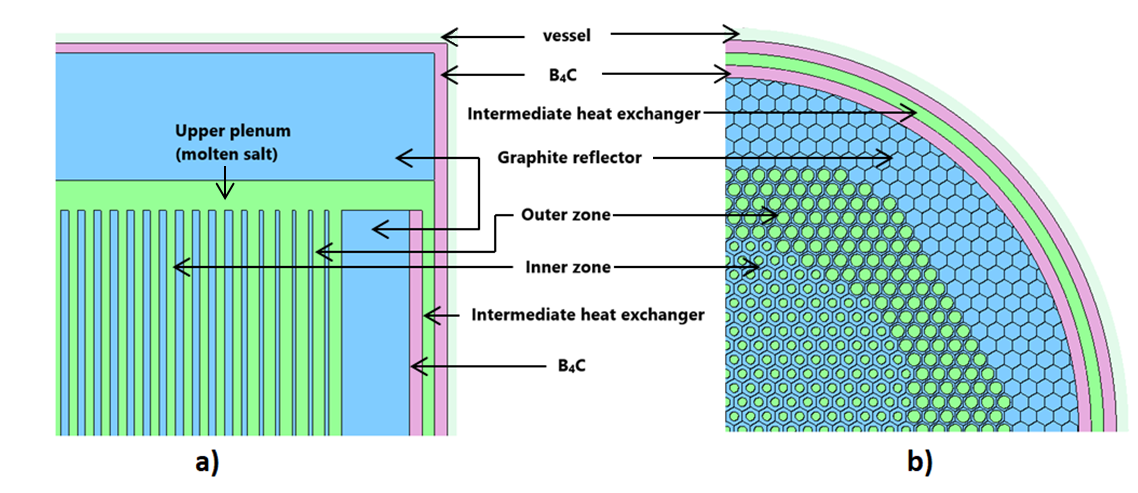
\includegraphics[width=\textwidth]{ff.png}
	\caption{$XZ$ (a) and $XY$ (b) section of the quarter-core model of the 
		SD-TMSR \cite{ashraf2019Preliminary}.}
	\label{fig:ff}
\end{figure}
In this study, the fuel salt composition is LiF-BeF$_2$-(HM)F$_N$ (70-17.5-12.5 mol\%),
where HM is the heavy metal (i.e. $^{232}$Th and fissile 
materials), and $N$ depends on the chosen fissile material and the 
thermochemical state of the liquid fuel salt. Three different types of initial 
fissile materials are considered: (1) $^{233}$U \cite{ashraf2020whole}, 
(2) reactor-grade Pu \cite{marka1993explosive}, and (3) transuranic (TRU) 
elements from \gls{LWR} \gls{SNF} \cite{de2000scenarios}.
The density and volume of the fuel salt are 3.3 g/cm$^{3}$ and 52.9 m$^3$, 
respectively. The liquid fuel salt circulates continuously through the channels
that pierce the graphite hexagonal prisms. The core is surrounded by 
axial and radial graphite reflectors to minimize the neutron leakage.
A 10-cm-thick B$_4$C cylinder surrounds the core to shield against neutrons and heat.
Finally, the SD-TMSR pressure vessel holds all reactor components and is made of 
a Hastelloy N alloy. The main characteristics of the SD-TMSR are 
summarized in Table~\ref{tab:table1}.


\begin{table}  %[!ht]
	\caption{The main characteristics of the SD-TMSR \cite{li_optimization_2018,ashraf2020whole}.}
	\vspace{0.1in}
	\begin{tabularx}{\textwidth}{l | r}
		\hline
		Thermal power, MW$_{th}$          				&  2,250  \\ 
		Fuel salt components                            & LiF-BeF$_2$-(\gls{HM})F$_N$ \\
		Fuel composition, mole\%                        & 70-17.5-12.5    \\
		$^7$Li enrichment, \%        				& 99.995   \\
		Fuel temperature, K 							& 900  \\
		Dilatation coefficient, g/(cm$^3$$\cdot{}$K)  &  -6.7$\times$10$^{-4}$ \\ 
		Fuel volume, m$^3$  &	52.9 \\
		Fuel density at 900 K, g/cm$^3$		  		& 3.3 \\
		Graphite density, g/cm$^3$             	    & 2.3	\\ 
		Core diameter, cm								& 460  \\
		Core height, cm									& 460  \\
		Side length of the graphite hexagonal prism, cm   & 7.5 \\
		Radius (inner fuel channel), cm							& 3.5  \\
		Radius (outer fuel channel), cm							& 5  \\
		Volume ratio of molten salt to graphite \\in the inner zone	&  0.357  \\
		Volume ratio of molten salt to graphite \\in the outer zone &  1.162  \\
		
		\hline
	\end{tabularx}
	\label{tab:table1}
\end{table}
%%%%%%%%%%%%%%%%%%%%%%%%%%%%%%%%%%%%%%%%

\subsection{Control rod design} \label{CRD}

The present paper proposes two sets of rods to control the reactivity of the SD-TMSR core:
\begin{enumerate}
\item Control Safety Devices (CSD);
\item Shutdown Safety Devices (SSD).
\end{enumerate}
The CSD system is designed for reactivity control during normal operation and the SSD system is designed for an emergency reactor shutdown.
In the present work, six different absorbing materials are considered based on their neutronics and safety performance:
\begin{enumerate}
\item natural B$_4$C (19.9\% $^{10}$B);
\item B$_4$C (enriched to 90\% $^{10}$B);
\item hafnium diboride (HfB$_2$);
\item hafnium hydride (HfH$_{1.62}$);
\item gadolinium oxide (Gd$_2$O$_3$);
\item europium oxide (Eu$_2$O$_3$).
\end{enumerate}

\begin{figure}[t!]  % replace 't' with 'b' to \centering
	\centering
	\hspace{+0.65in} 
	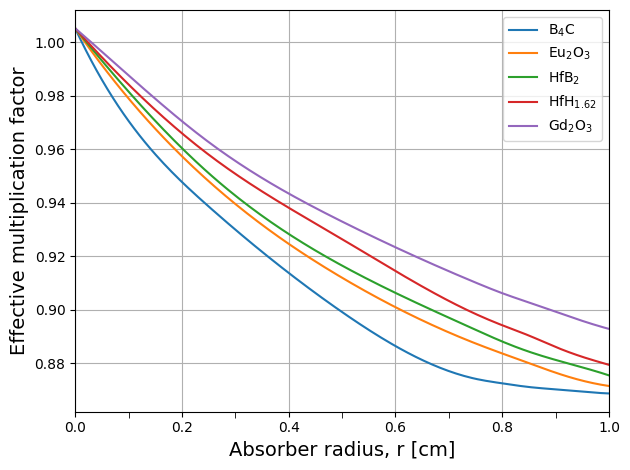
\includegraphics[width=\textwidth]{Radius.png}
	\caption{The change of the effective multiplication factor with the radius of the B$_4$C control rod.}
	\label{fig:Radius}
\end{figure}

The assessment of the optimal absorber radius should be an important consideration. If the CR radius is too large, the absorber material is not effectively utilized, due to self-shielding. We changed the radius of the CR and calculated the corresponding $k_{eff}$ when all CRs were fully inserted. Figure~\ref{fig:Radius} illustrates the change of the $k_{eff}$ with the radius of the B$_4$C control rod. As shown in Figure~\ref{fig:Radius}, in the region between 0 and 0.75 cm, the $k_{eff}$ decreases sharply with increasing absorber radius. However, in the region between 0.75 and 1.0 cm, there is almost no change in the $k_{eff}$. This is because of the geometry self-shielding of the neutron flux; beyond r = 0.75 cm, the $^{10}$B atoms in the central zone of the CR have relatively low chance for neutron capture.
From the obtained results, the control rod is a cylinder with a radius of 0.75 cm and a height of 520 cm. 
The absorbing material is surrounded by a 0.25-cm-thick cladding made of AIM1 
(15Cr-15Ni) steel alloy \cite{SERAN2017285} and the guide tube is made of 
SiC structural material (see Figure~\ref{fig:cr}). We simulated a 0.1-cm-thick gap between the 
cladding and guide tube to facilitate the control rod movement.
All densities of rod materials are listed in
Table~\ref{tab:table111}.

\begin{table}
	\caption{The densities of the absorbing materials.}
	\vspace{0.05in}
	\begin{center}	
		\begin{tabular}{|l | r|}  %[!ht]
			%%	\begin{tabularx}{\textwidth}{l | r}
			\hline
			Absorbers & Density [g/cm$^3$]\\
			\hline
			B$_4$C   &  2.54 \\
			HfB$_2$   &  10.5 \\
			HfH$_{1.62}$  &  11.4 \\
			Gd$_2$O$_3$   &  7.04 \\
			Eu$_2$O$_3$  &  7.38 \\
			SiC   & 3.21 \\
			AIM1 cladding   & 7.987 \\
			\hline
			%	\end{tabularx}
		\end{tabular}
		\label{tab:table111}
	\end{center}
\end{table}

%From the figure it can be seen that in the outer region of the B4C
%absorber, the flux is degraded rapidly, but in the region between 0 and 2 cm there is almost no change of the neutron flux. This phenomenon can be explained by the geometry self-shielding of the neutron flux. Due to absorption of low energy neutrons at the outside region ofthe absorber pin, the radius ofthe investigated pin is significantly larger than the penetration distance of the neutrons in the absorber. Therefore, the 10B atoms in the central part of the pin have no reasonable chance for neutron capture. Based
%
%
%On the basis of the obtained results the 5 ring configuration was selected for further
%ness (low self-shielding) and simplicity. On the basis of the obtained results the 5 ring configuration was selected for further
%analyses.
%
%This CR design consists of 61 absorber pins. Using Eq. (6) the radius of the absorber pins was calculated to 0.574 cm.
%
%In terms of neutronics, we an appropriate way to find the optimal pin radius could be the investigation of the neutron penetration distance, performed on a simple absorber pin.
%
%A single-pin design is a semi 1D approach preventing any interference caused by the self-shielding or geometrical influences of the surrounding absorber pins.

\begin{figure}[t!]  % replace 't' with 'b' to \centering
	\centering
	\hspace{+0.65in} 
	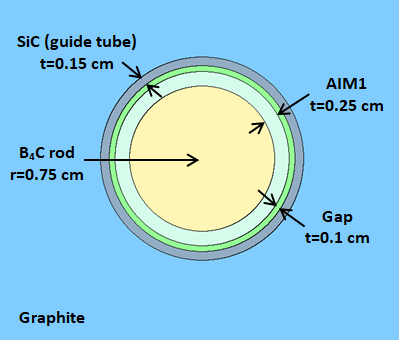
\includegraphics[width=\textwidth]{cr.png}
	\caption{Cross section of the B$_4$C control rod.}
	\label{fig:cr}
\end{figure}

Since the total number and distribution of the control assemblies in the SD-TMSR have not been determined, we propose an original distribution as a starting point of this analysis. We added clusters consisting of four control rods to specific graphite hexagonal prisms (elements) in the SD-TMSR core. Every four control rods can move together as one group (cluster). Figure~\ref{fig:graphite_elemen} demonstrates the plan view of the graphite element with the control rods. We propose 25 graphite elements with control rods: 16 Control Safety Devices (CSD) and 9 Shutdown Safety Devices (SSD).

\begin{figure}[t!]  % replace 't' with 'b' to \centering
	\centering
	\hspace{+0.65in}
	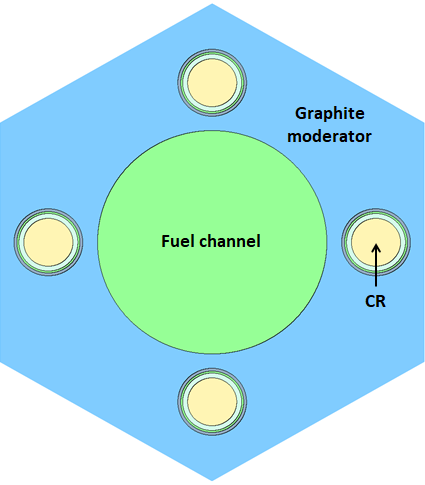
\includegraphics[width=\textwidth]{graphite_element.png}
	\caption{$XY$ section of graphite element with the four control rods 
	(cluster) located at the same distance from the fuel channel.}
	\label{fig:graphite_elemen}
\end{figure}
%\begin{figure}[t!]  % replace 't' with 'b' to \centering
%	\centering
%	\hspace{+0.65in}
%	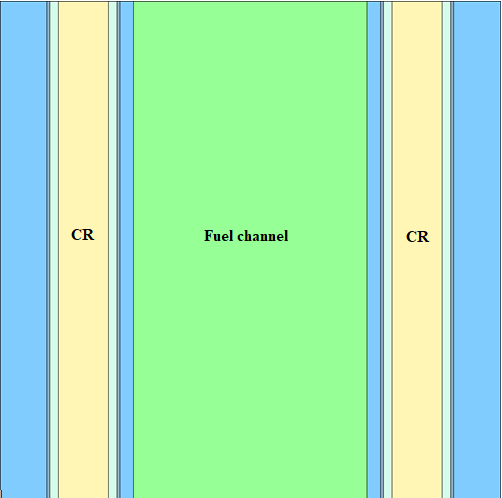
\includegraphics[width=\textwidth]{graphite_element1.png}
%	\caption{$XZ$ section of graphite element with control rods.}
%	\label{fig:graphite_elemen1}
%\end{figure}

Figure~\ref{fig:core_25} illustrates the numbering scheme of control rod 
clusters in the SD-TMSR core.
The CSD1-16 clusters are represented as yellow and distributed as two rings: inner and outer (peripheral) ring. The inner ring includes CSD from 1 to 6, while the outer ring includes CSD from 7 to 16. Red stands for SSD1-9 clusters.
We distributed the graphite elements with control rod clusters uniformly in 
the inner core of the SD-TMSR, in which the moderator-to-fuel ratio is high.
The selected core segment at the upper left corner of 
Figure~\ref{fig:core_25} shows that both CSD and SSD clusters consist of four 
control rods located at the same distance from the fuel channel center.
\begin{figure}[t!]  % replace 't' with 'b' to \centering
	\centering
	\hspace{+0.65in}
	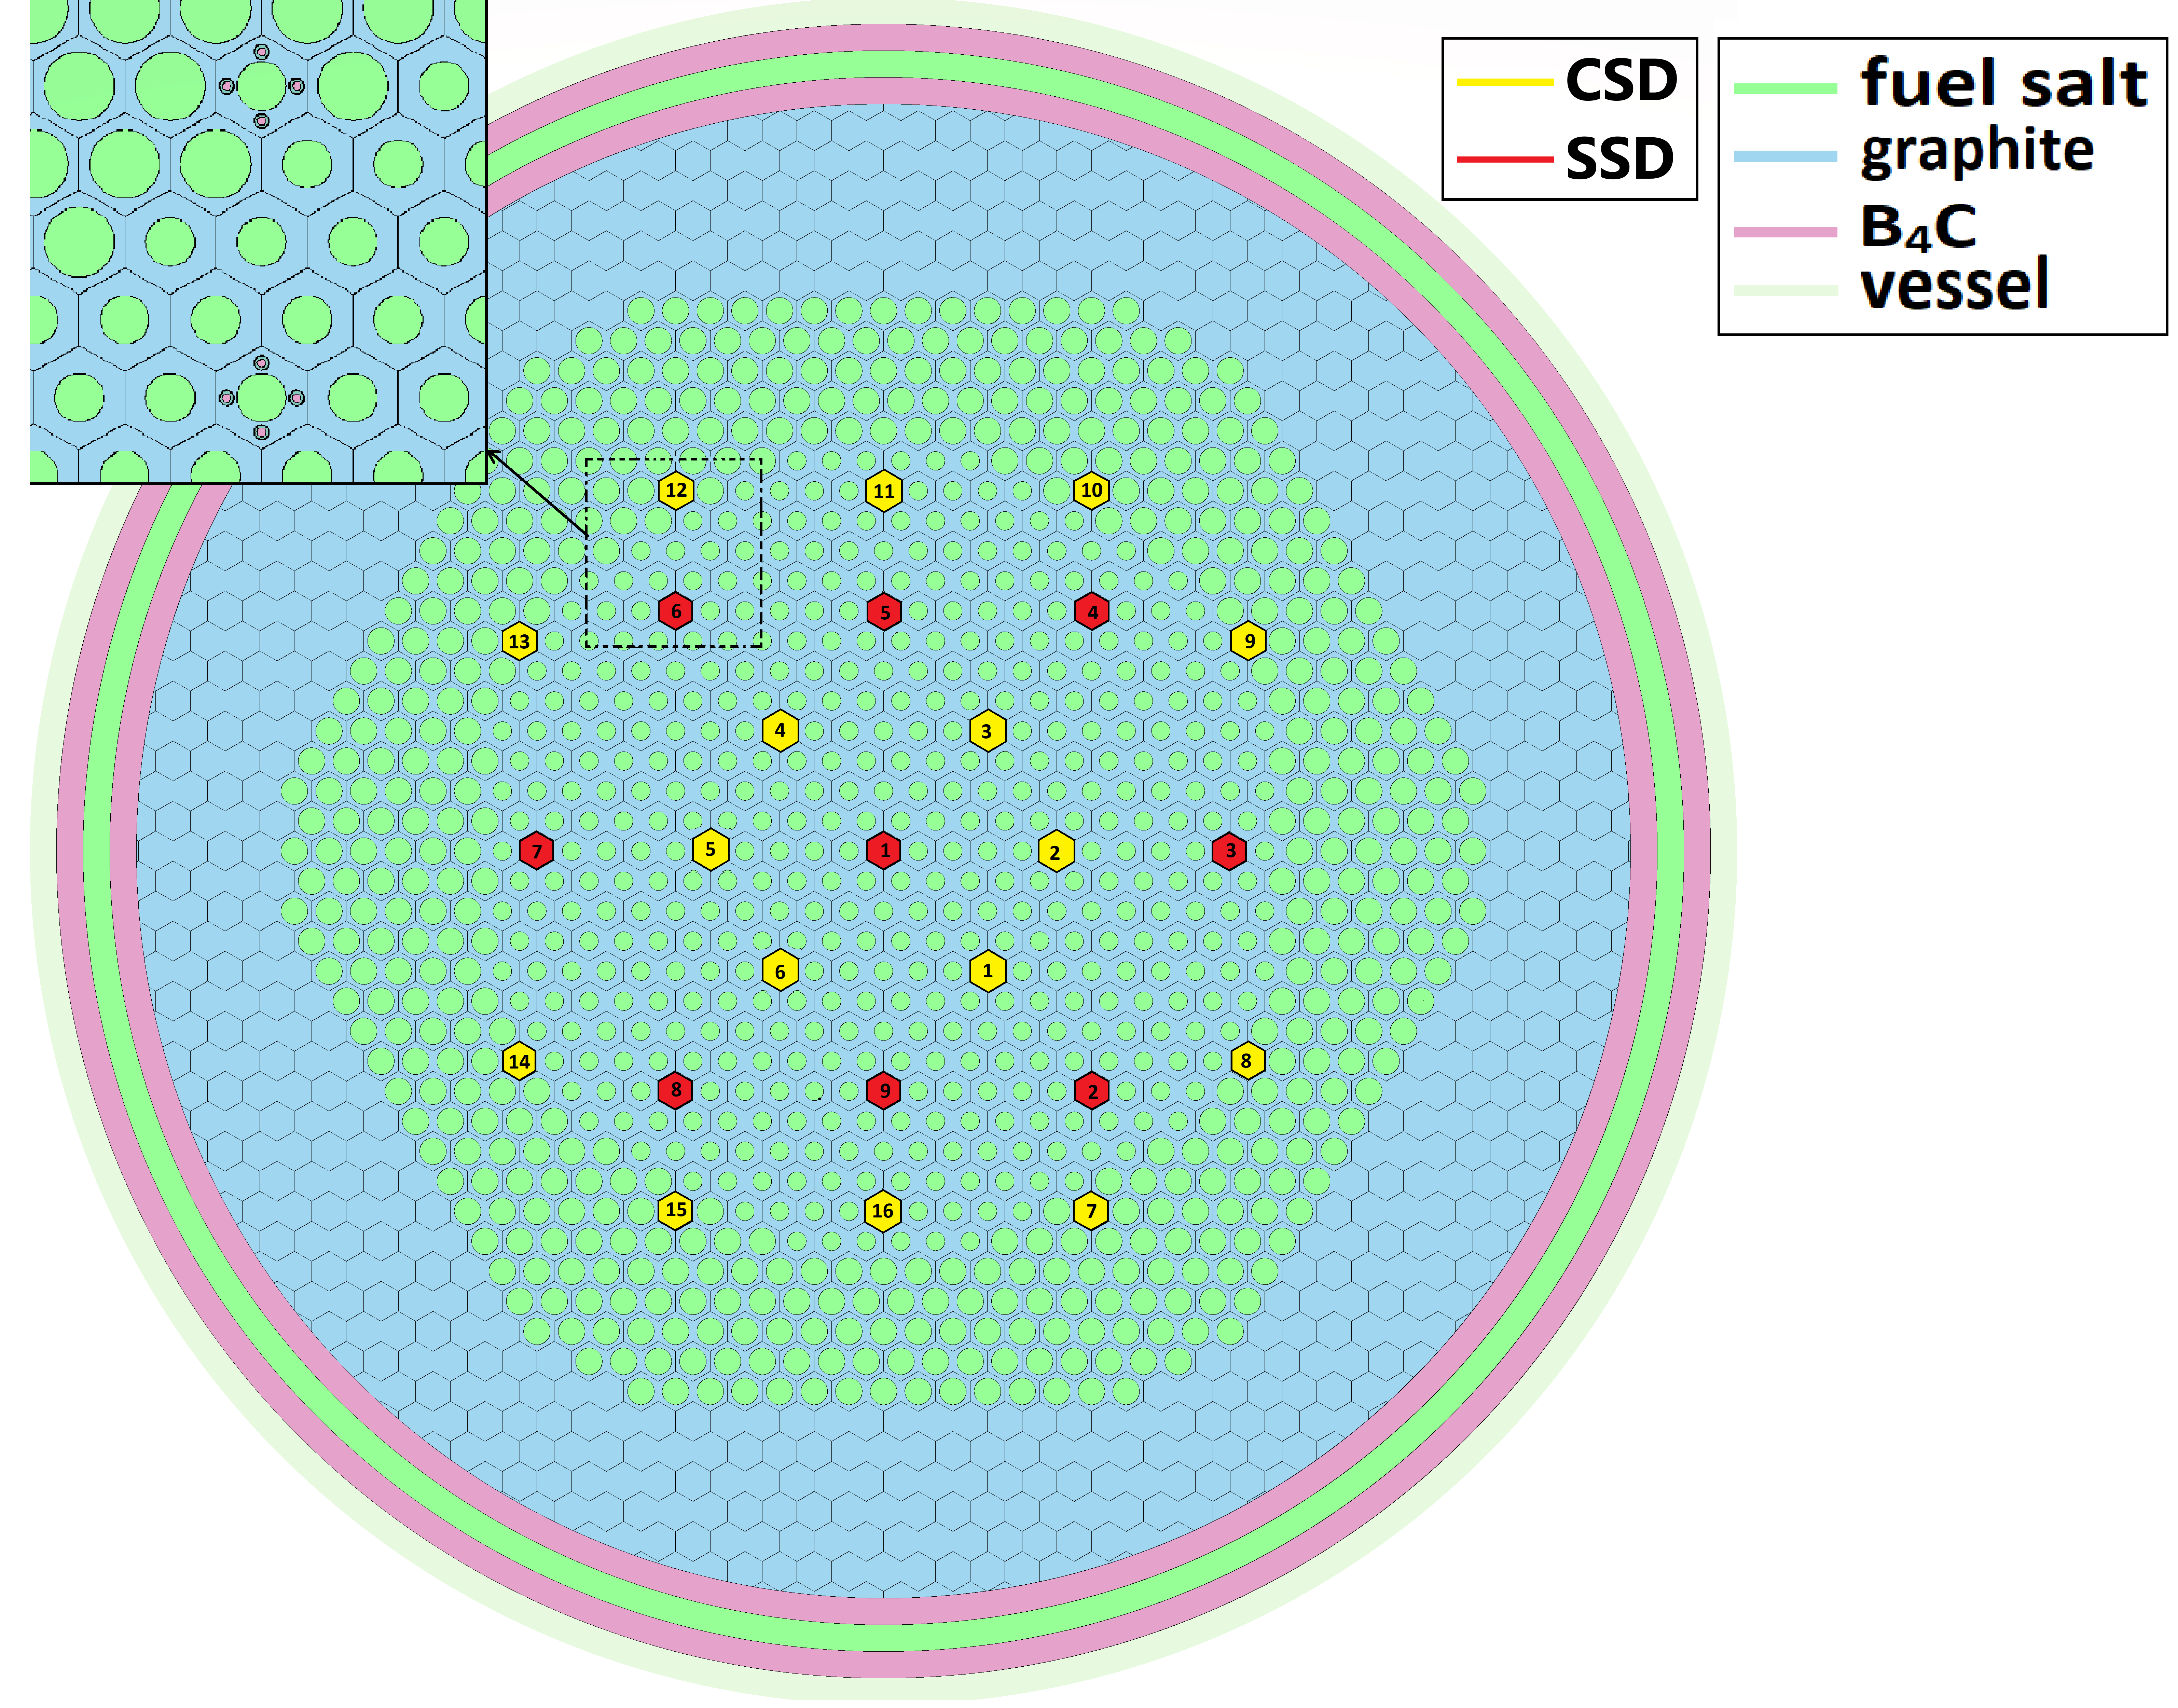
\includegraphics[width=\textwidth]{core_25.png}
	\caption{Distribution of the graphite elements with CRs in the SD-TMSR core.}
	\label{fig:core_25}
\end{figure}

\section{Methodology and tools} \label{Methodology-and-tools}
\subsection{Control rod design evaluation}
In this work, SERPENT-2 \cite{leppanen2014serpent} is used to 
perform steady state calculations for the full core of the SD-TMSR with 
the suggested control rod design. We adopted the ENDF-VII.0 cross section library 
for all calculations in the present work. The results demonstrated in this study were obtained after full-core calculations simulating 25$\times$10$^6$ active neutron histories per cycle. Simulations consisted in 500 active cycles of 5$\times$10$^4$ neutrons subdivided in 8 parallel tasks. Each simulation skipped 50 inactive cycles before beginning active tallies to allow for the convergence of the fission source distribution. Convergence has been checked through the fission source entropy. The statistical error in $k_{eff}$ was $\leq$ $25$ $pcm$.

%The results demonstrate whole-core runs of $50,000$ neutrons per cycle, for 50 inactive and 500 active cycles, and statistical error in $k_{eff}$ of $\leq$ $25$ $pcm$.
%
%Simulations consisted in 500 active cycles of 2∙104 neutrons. 20 inactive cycles were used for the convergence of the
%fission source distribution.
%
%Each simulation in this study skipped 200 generations before beginning active tallies to ensure fission source convergence.
%
%In order to minimize statistical errors and assure reliable fission source convergence, up to 2000 active fission source iteration cycles with 150,000 histories per cycle were used in neutron transport calculations with MCNP
%
%The MCNP transport step within the VESTA simulation uses 300 active cycles, 50 inactive cycles,
%and 100,000 particles per cycl
%
%The fission source defined in Serpent Code automatically dis-
%tributes the initial guess in fuel zones, with enhances the overall performance. Besides, the number of histories was selected to get the intended statistical convergence, considering the computa- tional effort involved. Accordingly, the following scheme was selected:
%? A Source with v3 ? 108 histories was selected for all cases where CRW is calculated in order to reach a statistical uncer- tainty of v5 pcm at 1 r for each calculation and a final value of CRW uncertainty below 5%.
%? A Source with v2 ? 107 histories was selected for all burnup cases in order to reach a statistical uncertainty of v20 pcm at 1 r for each calculation.
%3.3.
%
%The results presented in the following were obtained after full-core calculations simulating 250 million active neutron histories with the version 1.1.16 of the code. Simulations consisted in 500 active cycles of 5∙105 neutrons subdivided in 16 parallel tasks. Seventy inactive cycles were adopted to allow for the convergence of the fission source distribution. Convergence has been checked through the fission source entropy. Results

The initial calculation state of the SD-TMSR is identified by normal operation 
conditions (see Table~\ref{tab:table1}) and fully withdrawn control rod 
clusters. In this case, the control rods are located above the upper plenum as 
shown in Figure~\ref{fig:core_26}. To validate the proposed control rods 
system we adopted the same operation conditions (as in the initial calculation 
state) and changed the position of the control rod clusters along the $Z$ 
direction. The main calculated parameters including reactivity, control rod 
worth, and interference effects (shadowing effects) are described below.

\begin{figure}[t!] % replace 't' with 'b' to \centering
	\centering
	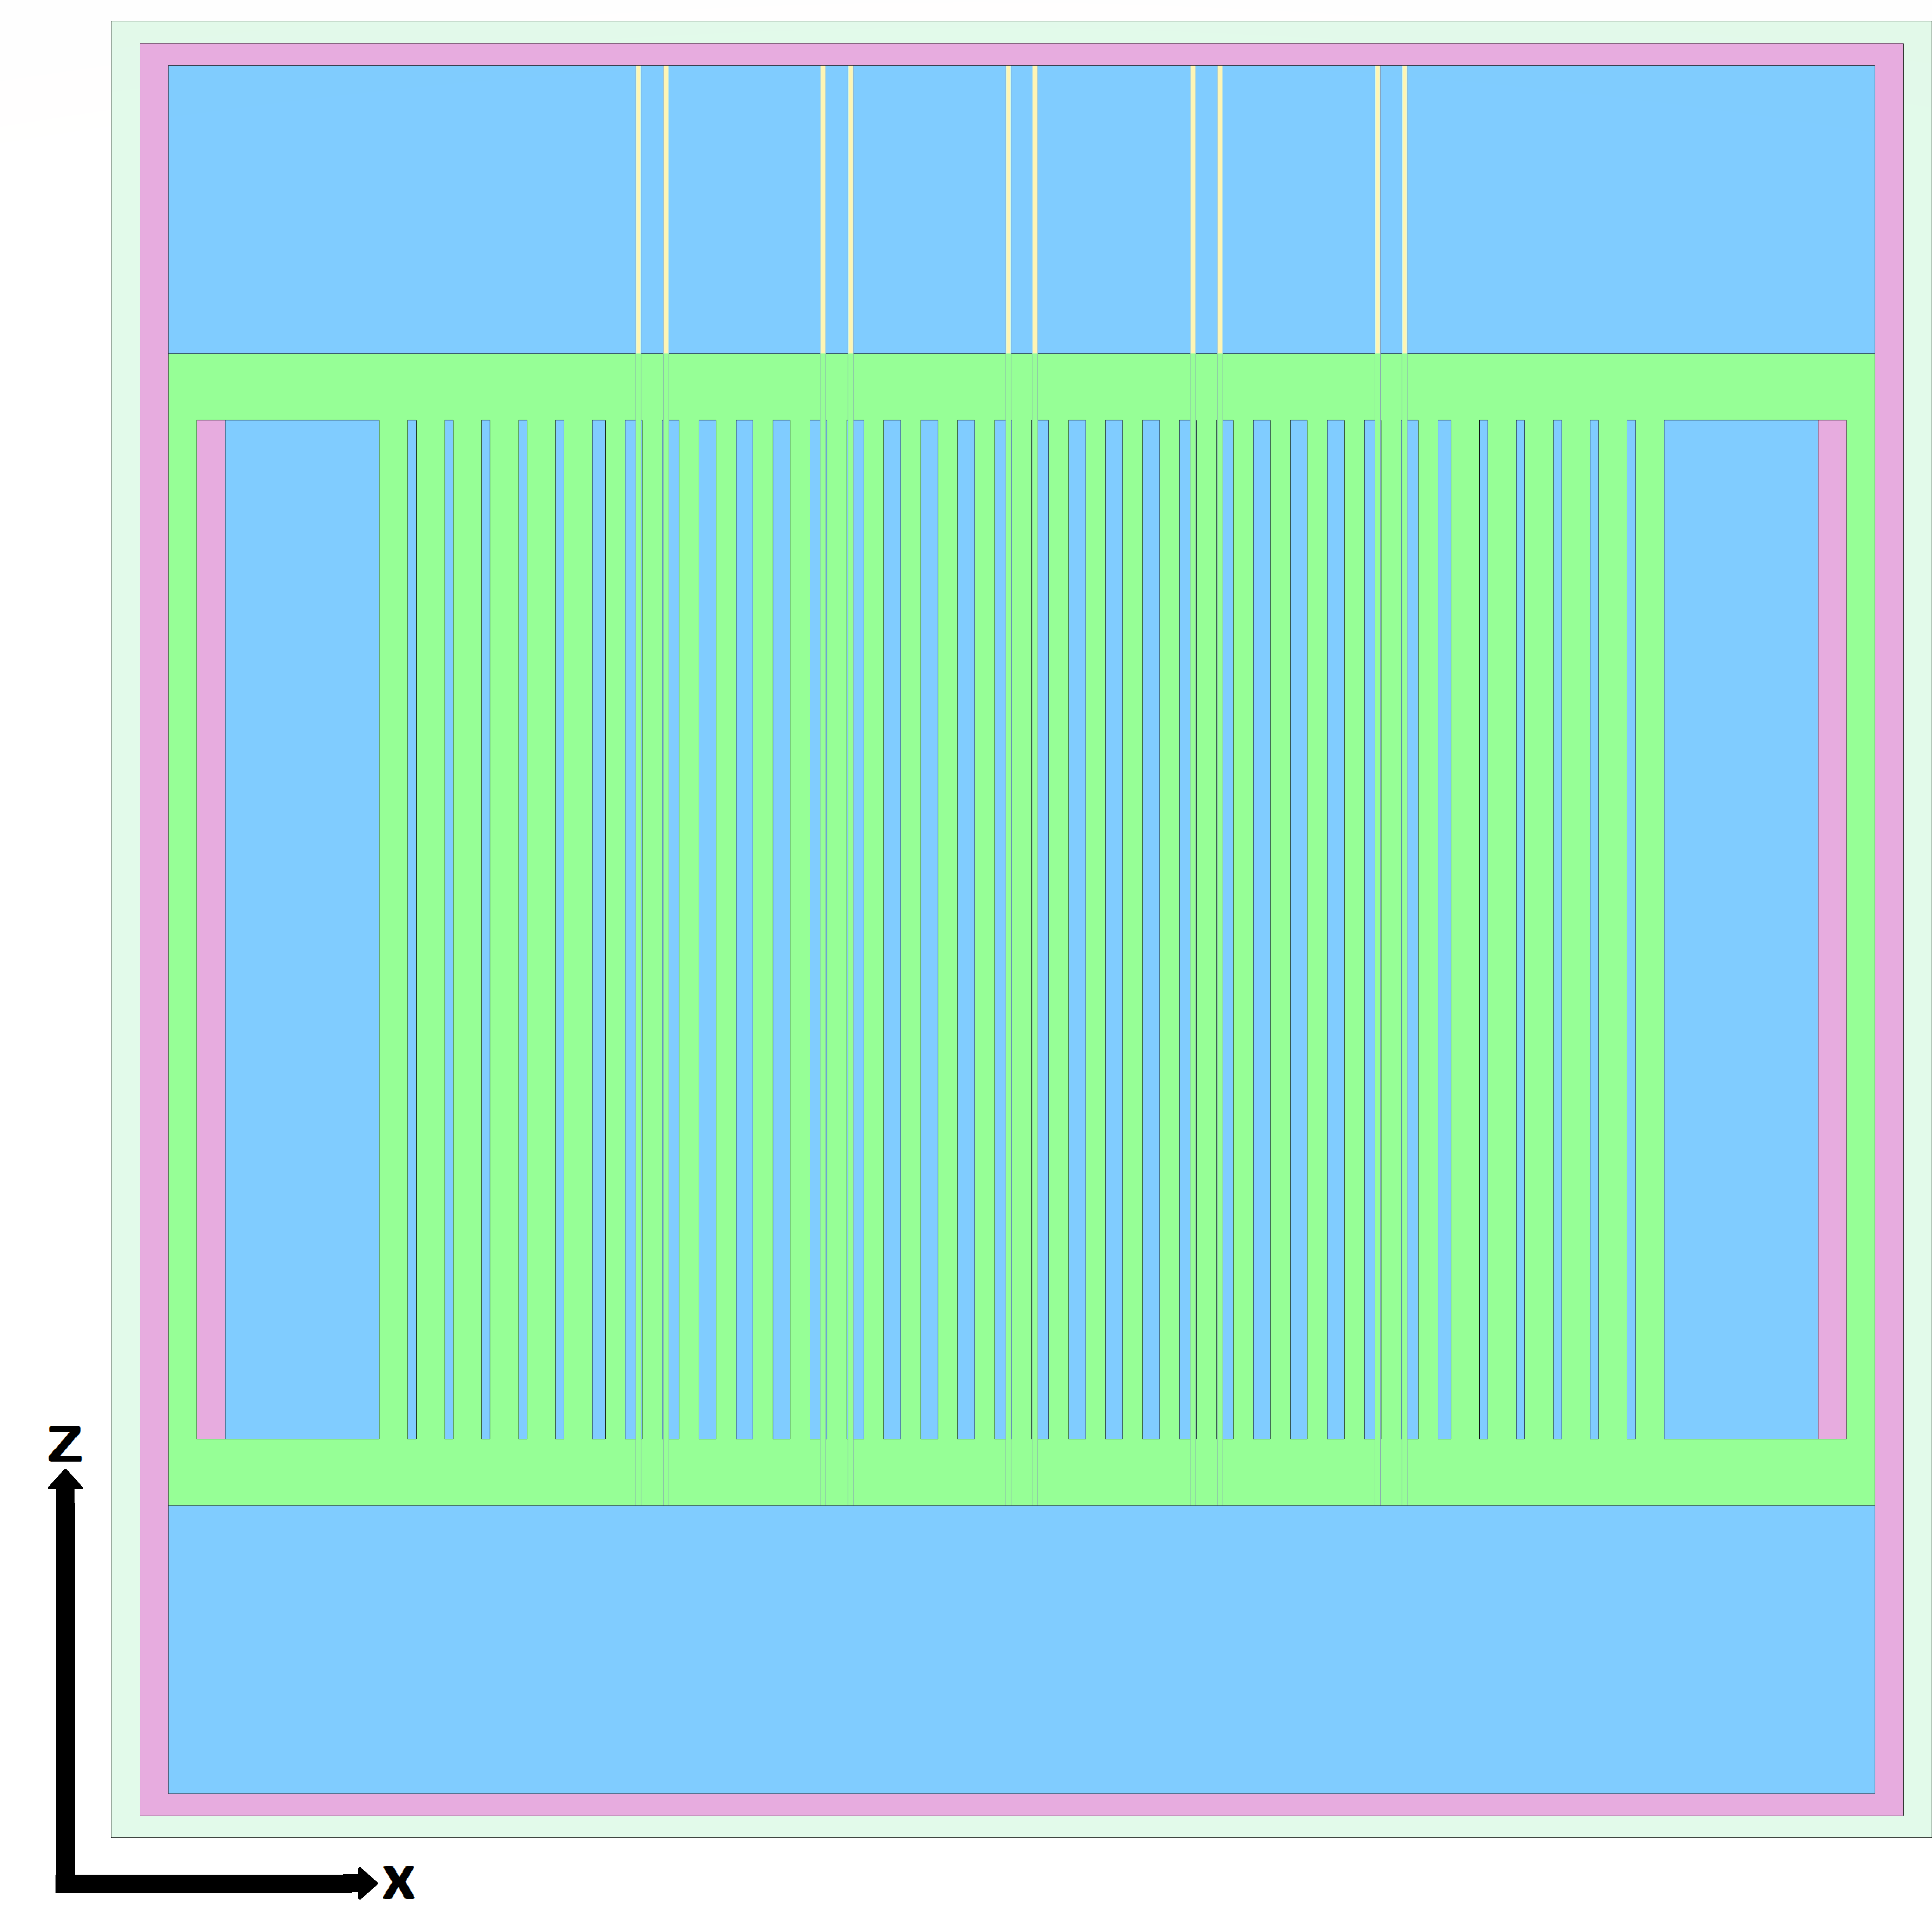
\includegraphics[width=\textwidth]{core_26.png}
	\caption{$XZ$ view at the midplane of the full-core model of the SD-TMSR, 10 CRs are fully withdrawn.}
	\label{fig:core_26}
\end{figure}

\subsubsection{Reactivity calculation}

The excess reactivity $\rho$$_e$ is the reactivity of the core when all control rods are withdrawn. $\rho$$_e$ is calculated by SERPENT-2 in \$ units based on equation~\ref{Equ:1}, where $k_{eff}$ is the effective multiplication factor of the core and $\beta_{eff}$ is the effective fraction of delayed neutrons:

\begin{equation}
\label{Equ:1}
{{\rho}_{e}}=\dfrac{{k_{eff}}-1}{{k_{eff}}{{\beta}_{eff}}}.
\end{equation}

The effective delayed neutron fraction is calculated by the adjoint-weighted time constants using a perturbation technique in SERPENT-2 \cite{leppanen2014calculation} and it accounts for the steady state of the fuel salt.

\subsubsection{The control rod worth (CRW)}

The control rod worth (CRW) is the amount of negative reactivity associated with the control rod insertion. The CRW is calculated by SERPENT-2 in \$ units based on equation~\ref{Equ:2}, where $\Delta\rho$$_{CRi}$ is the worth of the i$^{th}$ control rod (CR), $\rho$$_e$ is the initial excess reactivity, and $\rho$$_{CRi}$ is the excess reactivity after insertion of the i$^{th}$ CR \cite{vcerba2017optimization}:

\begin{equation}
\label{Equ:2}
{{\Delta}{\rho}_{CRi}}={{\rho}_{e}}-{{\rho}_{CRi}}.
\end{equation}

\subsubsection{Shutdown margin (SDM)}

The shutdown margin (SDM) is the amount of reactivity by which a full reactor core is subcritical from a given state. The Shutdown Safety Devices (SSD) clusters are designed mainly for an emergency shutdown, thus it should 
provide the reactor core with sufficient negative reactivity. The SDM is expressed in terms of reactivity and calculated by equation~\ref{Equ:6}, where $\Delta\rho_{SSD}$ is the total worth of the Shutdown Safety Devices (SSD) and $\rho$$_e$ is the core excess reactivity:

\begin{equation}
\label{Equ:6}
{SDM}={{\Delta}{\rho}_{SSD}}-{{\rho}_{e}}.
\end{equation}

\subsubsection{Interference effects (shadowing effects)}

Interference between control rods (CRs) or shadowing effects occur when one 
(or more) control rod impacts the reactivity worth of another control rod in 
the surroundings. 
The insertion of a CR depresses the neutron flux
in its vicinity and makes the curvature of the neutron flux greater. The gradient
of the neutron flux will contrarily increase at a radial distance. The CRs, distributed in the core,
will distort the neutron flux around each other and will impact the reactivity worth.
The term ``shadowing effect" has been used to describe this \cite{oka2014nuclear}.
The shadowing effect appears when the combined rod worth
is less than the sum of the individual worths. Meanwhile, anti-shadowing is observed 
when the combined rod worth is greater than the sum of the individual worths.
The core height-to-diameter ratio (H/D), CR locations, and the three-dimensional configuration 
of the CRs affect the degree of the interference between CRs \cite{oka2014nuclear}. 

The amplification factor of the i$^{th}$ CR (A$_{CRi}$) helps to evaluate the shadowing effects between CR clusters. The A$_{CRi}$ is calculated by equation~\ref{Equ:3} \cite{vcerba2017optimization}, where $\Delta\rho$$_{CR(1,2,\ldots N)}$ is the total worth of all CRs (from $1$ to $N$), $\Delta\rho$$_{CR(1,2,\ldots N-i)}$ is the total worth of all CRs except the i$^{th}$ rod, and $\Delta\rho$$_{CRi}$ is the worth of the i$^{th}$ rod:

\begin{equation}
\label{Equ:3}
{{A}_{CRi}}=\dfrac{{{\Delta}{\rho}_{CR(1,2,\ldots N)}}-{{\Delta}{\rho}_{CR(1,2,\ldots N-i)}}}{{\Delta}{\rho}_{CRi}}.
\end{equation}

If A$_{CRi}$ is $<$1, the CRW is reduced due to shadowing effects, but if A$_{CRi}$ is $>$1, the CRW is amplified and anti-shadowing effects occur \cite{girardin2007control}. A$_{CRi}$ = 1 means no shadowing effects occur.

\subsubsection{Integral and differential control rod worth}

The integral CRW is the total reactivity change due to the full 
insertion or withdrawal of the CR. However, the \textit{differential CRW} is the
reactivity inserted per unit of withdrawal [\$/cm]. To calculate those 
parameters, we varied the position of CR clusters from fully withdrawn to 
fully inserted. Equation~\ref{Equ:4} is used to calculate the integral CRW 
[\$], where $k_{j-1}$ and $k_{j}$ are the effective multiplication factors 
before and after CR insertion to the $j$$^{th}$ step, respectively, $\beta_{j}$ is the
fraction of delayed neutrons at the $j$$^{th}$ step, and $N$ is the number of steps:

\begin{equation}
\label{Equ:4}
{{\Delta}{\rho}_{j}}=\sum_{j=1}^{N}\dfrac{{k_{j}}-{k_{j-1}}}{{{k_{j}}{k_{j-1}}}{{\beta}_{j}}}.
\end{equation}

Equation~\ref{Equ:5} is used to calculate the differential CRW, where 
$\Delta Z$ is the length of rod inserted:

\begin{equation}
\label{Equ:5}
\dfrac{{\partial}{\rho}_{j}}{{\partial{Z}}}=\dfrac{1}{{\Delta}{Z}}\dfrac{{k_{j}}-{k_{j-1}}}{{{k_{j}}{k_{j-1}}}{{\beta}_{j}}}.
\end{equation}



\FloatBarrier
\section{Results and discussion} \label{Results-and-discussion}

The SERPENT-2 is used to obtain the presented results.
We use the ENDF-VII.0 cross section library for all calculations in the current work. The statistical error in $k_{eff}$ is $\leq$ $25$ $pcm$.
The initial calculation state of a full 3D model of the SD-TMSR is identified by normal operation 
conditions (see Table~\ref{tab:table1}) and fully withdrawn control rod 
clusters. 
To validate the proposed control rods 
system we adopted the same operation conditions (as in the initial calculation 
state) and changed the position of the control rod clusters along the $Z$ 
direction.
The obtained results including reactivity, control rod 
worth, and interference effects (shadowing effects) are discussed below.

\subsection{Excess reactivity}

The excess reactivity $\rho$$_e$ is calculated at zero burnup (steady-state 
calculation), when all control rods (CRs) are fully withdrawn. The $\rho_e$ for $^{233}$U, 
reactor-grade Pu, and TRU used as initial fissile material are listed in Table~\ref{tab:excess}.
For $^{233}$U case \cite{ashraf2020Strategies} the maximum observed excess reactivity is $4.27\pm0.01$ $\$$ during 60 effective full-power years (EFPY) of operation (see Figure~\ref{fig:keff_25} at $\approx$ 8 EFPY).
The proposed reactivity control system must compensate such reactivity at startup and during burnup.
\begin{figure}
	\centering
	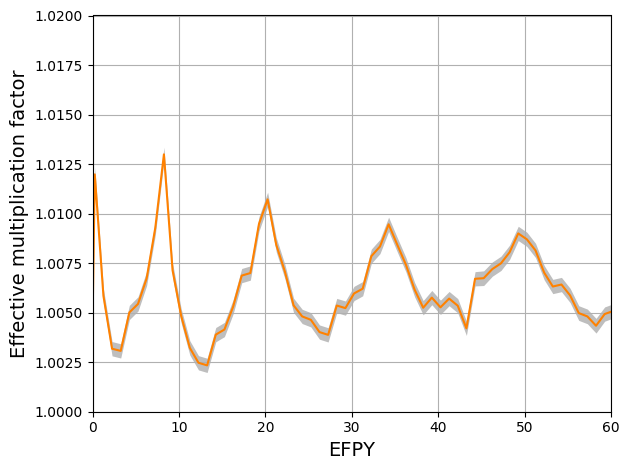
\includegraphics[width=\textwidth]{keff_25.png}
	\vspace{-0.5in}
	\caption{Uncontrolled effective multiplication factor during 60 EFPY of reactor operation
		including periodic $^{233}$U/$^{232}$Th insertion (confidence interval $\pm\sigma$ is shaded) \cite{ashraf2020whole}.} 
	\label{fig:keff_25}
\end{figure}

\begin{table}  %[!hb]
	\caption{The excess reactivity at startup for the SD-TMSR core with different initial fissile materials.}
	\vspace{0.1in}
	\begin{tabularx}{\textwidth}{p{3cm} s s s}
		\hline
		Initial fissile materials       				&  $^{233}$U & reactor-grade Pu&  TRU \\
		\hline
		$\rho_e$					& $1.65\pm0.04$ $\$$ & $4.11\pm0.02$ $\$$ & $15.38\pm0.04$ $\$$ \\
		\hline
	\end{tabularx}
	\label{tab:excess}
\end{table}

\subsection{Control rod parameters}

The control rod parameters including control rod worth (CRW), interference 
between CR clusters, and integral and differential control rod worths are 
described in this work. Table~\ref{tab:worth} shows calculated CRW and the amplification 
factor (A$_{CRi}$) for six different 
absorbers. The types of interference for all different 
absorbers are listed in Table ~\ref{tab:table25}. Fuel salt composition of LiF-BeF$_2$-ThF$_4$-$^{233}$UF$_4$ at 70-17.5-12.3-0.2 mole\% is used to generate the results listed in Tables~\ref{tab:worth} and ~\ref{tab:table25}.
\begin{sidewaystable}
	\fontsize{5}{7}\selectfont
	\centering
	\caption{The control rod worth for different CR 
		materials.}
	\vspace{1ex}
	\begin{tabularx}{\textwidth}{|p{1.8cm}|p{1cm}|p{1cm}|p{1cm}|p{1cm}| 
			p{1cm}|p{1cm}|p{1cm}|p{1cm}| 
			p{1cm}|p{1cm}|p{1cm}|p{0.9cm}|}
		\hline
		\multirow{2}{*}{Control Rod group}		& 
		\multicolumn{2}{c|}{Nat. B$_4$C} & \multicolumn{2}{c|}{B$_4$C-90}   	&\multicolumn{2}{c|}{HfB$_2$}	
		&\multicolumn{2}{c|}{HfH$_{1.62}$} 
		&\multicolumn{2}{c|}{Gd$_2$O$_3$}	& 	
		\multicolumn{2}{c|}{Eu$_2$O$_3$} \\
		\cline{2-13}
		& $\Delta\rho$$_{CRi}$  [\$]  &A$_{CRi}$	
		& $\Delta\rho$$_{CRi}$  [\$]  &A$_{CRi}$		
		&$\Delta\rho$$_{CRi}$ [\$]  &A$_{CRi}$		
		&$\Delta\rho$$_{CRi}$ [\$]	&A$_{CRi}$		
		&$\Delta\rho$$_{CRi}$ [\$]	&A$_{CRi}$		
		&$\Delta\rho$$_{CRi}$ [\$]	&A$_{CRi}$  \\
		\hline                   
		All control rods      &  $42.04\pm0.60$	&	& $48.19\pm0.68$   &		
		&$40.40\pm0.41$	&		&$37.96\pm0.36$	&		&$33.70\pm0.40$	&	
			&$42.39\pm0.48$	& 	 \\
		\hline 
		CSD 		 & $22.32\pm0.20$ 	& $1.24\pm0.01$	 			& $25.50\pm0.23$   &$1.24\pm0.01$	 	&$21.90\pm0.17$	&$1.10\pm0.01$	 	&$20.62\pm0.34$	&$1.10\pm0.01$	 	&$18.48\pm0.25$	&$1.17\pm0.01$	 	&$22.96\pm0.18$	&$1.20\pm0.01$   \\
		\hline 
		SSD		   & $14.27\pm0.10$ 	&$1.38\pm0.02$	 	&$16.39\pm0.11$ &$1.38\pm0.02$	 	&$14.27\pm0.21$	&$1.29\pm0.01$	 	&$13.23\pm0.18$	&$1.30\pm0.06$	 	&$12.00\pm0.20$	&$1.26\pm0.01$	 	&$14.58\pm0.11$	&$1.30\pm0.02$	  \\
		\hline 
		CSD inner ring   &  $16.80\pm0.02$	&$1.50\pm0.01$	  &  $18.42\pm0.05$  &$1.60\pm0.04$	 		&$16.29\pm0.29$	&$1.48\pm0.02$	 	&$15.50\pm0.17$	& $1.46\pm0.01$  	&$14.12\pm0.07$	&$1.39\pm0.01$	 	&$16.92\pm0.13$	&$1.50\pm0.01$	  \\
		\hline 
		CSD outer ring            &  $2.16\pm0.02$	&$3.11\pm0.06$	     &$2.26\pm0.02$ &$4.21\pm0.07$	 	&$2.10\pm0.06$	&$3.11\pm0.10$ 	&$1.85\pm0.07$	&$3.24\pm0.06$	 	&$1.80\pm0.10$	&$2.54\pm0.14$	 	&$2.14\pm0.05$	&$3.20\pm0.05$	  	\\
		\hline 
		CSD2			 &  $2.11\pm0.03$	&$3.00\pm0.08$	 			& $2.25\pm0.04$   &$3.69\pm0.16$	 	&$2.24\pm0.05$	&$2.42\pm0.10$	 	&$2.00\pm0.10$	&$2.68\pm0.03$	 	&$1.80\pm0.10$	&$2.55\pm0.20$	 	&$2.19\pm0.12$	&$2.90\pm0.08$	  \\
		\hline 
		CSD9			 &  $0.06\pm0.01$	&$15.16\pm0.10$	 				& $0.15\pm0.04$   & $10.53\pm0.01$	  	&$0.10\pm0.05$	&$5.10\pm0.05$	 	&$0.05\pm0.01$	&$16.40\pm0.10$	  	&$0.09\pm0.07$	&$5.55\pm0.20$	  	&$0.07\pm0.05$	&$14.00\pm0.10$	  \\ 
		\hline
		SSD1		 &  $3.95\pm0.05$	&$1.31\pm0.01$	 	& $4.18\pm0.07$   &$1.59\pm0.08$	 	&$3.95\pm0.13$	&$1.30\pm0.07$	 	&$3.59\pm0.03$	&$1.49\pm0.01$	 	&$3.45\pm0.12$	&$1.40\pm0.08$	 	&$3.91\pm0.06$	&$1.40\pm0.01$  \\
		\hline 
		SSD4		 &  $0.59\pm0.08$	& $9.52\pm0.10$	 		&  $0.57\pm0.09$  &$7.84\pm0.15$	 	&$0.63\pm0.06$	&$4.40\pm0.10$	 	&$1.00\pm0.05$	&$2.51\pm0.16$	 	&$0.60\pm0.80$	&$3.31\pm0.27$	 	&$0.60\pm0.08$	&$5.10\pm0.28$	  \\
		\hline
	\end{tabularx}
	\label{tab:worth}
\end{sidewaystable}

\begin{sidewaystable}
	\fontsize{5}{7}\selectfont
	\centering
	\caption{The shadowing effect for different CR materials.}
	\vspace{0.1in}
		\begin{tabularx}{\textwidth}{|X|X|X|X|X|X|X|}
		\hline
		\multirow{2}{*}{Control Rod group}		& Nat. B$_4$C & B$_4$C-90  	&HfB$_2$
		&HfH$_{1.62}$
		&Gd$_2$O$_3$& 	
		Eu$_2$O$_3$ \\
		\cline{2-7}
		&  Interference
		& Interference	
		& Interference	
		& Interference	
		& Interference
		& Interference \\
		\hline                   
	CSD 		&	$\star$				& $\star$	&$\star$		&$\star$		&$\star$  &$\star$	 \\
	\hline 
	SSD		   &	$\star$				& $\star$	&$\star$		&$\star$		&$\star$  &$\star$	 \\ 
	\hline 
	CSD inner ring   &  	$\star$				& $\star$	&$\star$		&$\star$		&$\star$  &$\star$	 \\
	\hline 
	CSD outer ring       &	$\star$				& $\star$	&$\star$		&$\star$		&$\star$  &$\star$	 \\     
	\hline 
	CSD2			&	$\star$				& $\star$	&$\star$		&$\star$		&$\star$  &$\star$	 \\  
	\hline 
	CSD9		&	$\star$$\star$				& $\star$$\star$	&$\star$		&$\star$$\star$			&$\star$$\star$	  &$\star$$\star$		 \\ 	 
	\hline
	SSD1	&	$\star$				& $\star$	&$\star$		&$\star$		&$\star$  &$\star$ \\	  
	\hline 
	SSD4		&		$\star$$\star$			& 	$\star$$\star$	&$\star$		&$\star$		&$\star$  &	$\star$$\star$	 \\  
	\hline
	\end{tabularx}
	\begin{tablenotes}
	\tiny
	\item  $\star$  anti-shadowing effects observed
	\item  $\star$$\star$ strong anti-shadowing effects observed
\end{tablenotes}
	\label{tab:table25}
\end{sidewaystable}
\subsubsection{CRW} \label{CR_worth}

Among the absorbers investigated, the total worth of all CRs extends from $33.7\pm0.4$ $\$$ to $48.19\pm0.68$ 
$\$$ (the first row in Table~\ref{tab:worth}). B$_4$C-90 (boron enriched to 90\% $^{10}$B)
has the largest absorption ability, while Gd$_2$O$_3$ has the lowest 
absorption compared with the other absorbing materials in this study. This 
result agrees with macroscopic absorption cross section data 
\cite{guo2019optimized}. B$_4$C-90 has the highest macroscopic 
absorption cross section followed by Eu$_2$O$_3$, natural B$_4$C (Nat. B$_4$C), HfB$_2$, HfH$_{1.62}$, and 
finally Gd$_2$O$_3$. The CR material is being transmuted during 
operation; the effect of the fuel salt burnup on the CRW is neglected
herein and will be investigated in future work.

The worth of the Control Safety Devices (CSD) clusters is $1.56$ times greater than 
the worth of the Shutdown Safety Devices (SSD) system for all absorbing materials. Either CSD or SSD 
clusters are able to shut down the reactor initially loaded by 
$^{233}$U and reactor-grade Pu regardless the absorbing material type.
However, only SSD clusters made of B$_4$C-90 are able to shut down the SD-TMSR 
initially loaded by transuranic (TRU) elements ($\rho_e$ is $15.38\pm0.04$ $\$$).
The reason for this is the much larger 
absorption cross section of $^{10}$B in the relatively soft neutron energy 
spectrum of the SD-TMSR core started with TRU \cite{ashraf2020Strategies}.

The inner ring of the CSD is located in the central zone of the SD-TMSR core 
(Figure~\ref{fig:core_25}), in which the volume ratio between molten salt and 
graphite is relatively small ($0.357$). Results show that the inner ring of the CSD has 
a worth almost equal to the worth of all other CRs together (SSD + CSD outer ring) regardless of 
the absorbing material type (see Table~\ref{tab:worth}). This happens because the absorption cross section
decreases with the energy of the incident neutron; for example, boron absorbs neutrons in the thermal spectrum much 
greater than in the fast spectrum. Additionally, the maximum neutron flux is located in the central zone of the SD-TMSR (see Figure~\ref{fig:totalflux}); therefore, the inner ring of the CSD has a worth higher than the worth of the outer ring of the CSD.

In case of malfunction of other CR clusters (e.g., stuck in the upper 
position), the outer ring of the CSD will be able to compensate the excess reactivity of the core initially loaded by $^{233}$U.
Meanwhile, it will fail to compensate the excess 
reactivity of the core initially loaded by reactor-grade Pu and TRU elements. In this unlikely case, the fuel salt temperature will rise, melt a freeze plug, and hot salt will be drained into subcritical drain tanks to safely shut down the reactor.

We separately calculated the worth of CSD2, CSD9, SSD1, and SSD4 clusters (i.e., clusters located in the center and at the boundary between the core
zones, see Figure~\ref{fig:core_25}) to investigate the variation of CRW with the position in the inner core.
The CRW decreases in the direction of the outer core zone. The outer core zone 
has smaller moderator-to-fuel ratio ($0.86$) compared with the central zone 
($2.8$); consequently, the neutron energy spectrum is faster in the peripheral 
zone than in the center of the core degrading the CR's 
absorption ability in that region.

\subsubsection{Shutdown margin (SDM)}

The Shutdown Safety Devices (SSD) clusters are designed mainly for an emergency shutdown, thus it should 
provide the reactor core with sufficient negative reactivity. The 
shutdown margin (SDM) is calculated by equation~\ref{Equ:6}.
Table~\ref{tab:table2} summarizes the shutdown margins for the SD-TMSR core 
initially loaded with $^{233}$U, reactor-grade Pu, and TRU 
elements for different absorbing materials. All absorbing materials provide a sufficient positive
SDM for the SD-TMSR core that is initially loaded with 
$^{233}$U and reactor-grade Pu. However, the SDMs for the TRU case are 
negative or slightly positive (in B$_4$C-90 case); this makes the SSD clusters 
unreliable to shut down the reactor loaded with TRU.
As mentioned previously, the SSD clusters should 
provide a sufficient positive SDM.

\begin{table}  %[!hb]
	\caption{The SDMs for the SD-TMSR core for different absorbing materials.}
	\vspace{0.1in}
	\begin{tabularx}{\textwidth}{p{3cm} s s s}
		\hline
		Absorbing materials        				&  $^{233}$U & reactor-grade Pu&  TRU \\
		\hline
		Nat. B$_4$C					& $12.62\pm0.08$ $\$$ &$10.18\pm0.09$ $\$$ &$-1.12\pm0.08$ $\$$ \\
		B$_4$C-90                          & $14.74\pm0.09$ $\$$ & $12.28\pm0.12$ $\$$ & $ $ $ $ $1.01\pm0.09$ $\$$ \\
		Eu$_2$O$_3$                       &  $12.93\pm0.09$ $\$$    &  $10.47\pm0.12$ $\$$   &$-0.80\pm0.09$ $\$$\\
		HfB$_2$        				 &$12.62\pm0.24$ $\$$ &$10.16\pm0.26$ $\$$ &$-1.11\pm0.24$ $\$$   \\
		HfH$_{1.62}$							& $11.58\pm0.19$ $\$$ &$9.12\pm0.22$ $\$$ &$-2.15\pm0.19$ $\$$ \\
		Gd$_2$O$_3$	  		& $10.35\pm0.22$ $\$$ &$7.890\pm0.25$ $\$$& $-3.38\pm0.22$ $\$$\\
		\hline
	\end{tabularx}
	\label{tab:table2}
\end{table}

\subsubsection{Interference between CR systems}

The amplification factor (A$_{CRi}$) results show that the CSD, SSD, CSD inner 
ring, and SSD1 are slightly amplified due to the anti-shadowing effects. The 
anti-shadowing is observed when the combined rod worth is greater than the sum 
of the individual worths. As listed in Tables~\ref{tab:worth} and ~\ref{tab:table25}, the strongest anti-shadowing effect occurred in 
SSD4 and CSD9 clusters that are located at the boundary between the core zones 
with different moderator-to-fuel ratios. This can be attributed to the fact that the SSD4 and CSD9 clusters are surrounded by fewer clusters compared with other clusters located in the inner zone of the SD-TMSR (see Figure~\ref{fig:core_25}). Consequently, low interference between the SSD4 and CSD9 clusters and other surrounding clusters is observed. The obtained results show a negligible relationship between the absorbing material type and the interference between the CR clusters (i.e., the A$_{CRi}$).

Insertion of the CR affects the neutron flux distribution, which is 
the primary reason for the amplification of CRWs indicated in 
Table~\ref{tab:worth}. Figure~\ref{fig:totalflux} illustrates the radial 
neutron flux distribution at the mid-core level with different CR positions: 
(1) all CRs withdrawn, (2) all CRs inserted, (3) all CSD inserted, (4) all SSD 
inserted. We chose the B$_4$C-90 as the absorbing material because of its high 
absorption ability. As shown in Figure~\ref{fig:totalflux}, the insertion of 
CRs deforms the radial flux shape close to CRs.
This shifts the neutron flux from the core center towards the 
periphery. The maximum neutron flux shift occurs when all CRs are inserted 
into the core \cite{girardin2007control}.
\begin{figure}[!ht]
	\centering
	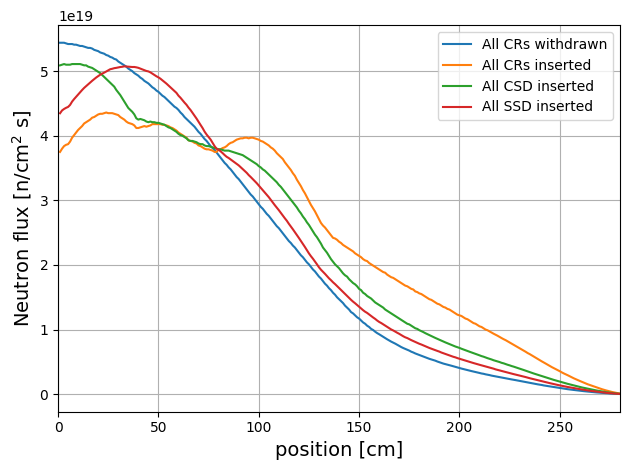
\includegraphics[width=\textwidth]{totalflux.png}
	\vspace{-0.5in}
	\caption{Radial neutron flux distribution at the mid-core for different 
	CR positions (CRs made of B$_4$C-90).} 
	\label{fig:totalflux}
\end{figure}
 

\subsubsection{Integral and differential CRW}

The integral and differential CRWs are calculated for three 
different systems: all CRs, CSD, and SSD systems. The CRs are 
inserted gradually into the core from the top to the bottom. 
Equations~\ref{Equ:4} and~\ref{Equ:5} are used to calculate the integral and 
differential CRW, respectively. Figure~\ref{fig:integ} illustrates the integral CRW for CRs 
made of B$_4$C-90. The maximum integral worth of all CRs, CSD, and SSD 
clusters are about $48.39$ $\$$, $25.30$ $\$$, and $16.46$ $\$$, respectively. The 
integral worth of SSD clusters made of B$_4$C-90 is sufficient to shut down the reactor from any 
state.

The differential CRWs are demonstrated in Figure~\ref{fig:diff}. Theoretically, at the top of the core, the CR insertion has little effect since this region has low thermal neutron flux. Thus the differential CRW has the lowest values in this region. The effect of CR insertion increases gradually near the center of the core. At the center of the core (region with maximum thermal neutron flux), the differential CRW is the largest and changes slowly with rod insertion. From the center of the core to the bottom, the differential CRW values decrease (region with low thermal neutron flux). Figure~\ref{fig:diff} shows that the maximum differential CRW is shifted toward the bottom of the core and the curves are not exactly symmetrical. This is due to the asymmetrical distribution of the fuel and graphite in simulation \cite{xuemei2013study,son2016control}.

Figure~\ref{fig:CSD} shows the integral CRW for only Control Safety Devices (CSD) clusters with six 
different absorbing materials. The results show that all absorbing materials 
have almost the same integral rod worth in the upper half of the core 
($<250$ cm from the upper boundary of the core). Further insertion of the 
CRs demonstrates that the strongest absorber, B$_4$C-90 outperforms other materials.
Notably, all results are based on steady-state calculations. 

\begin{figure}
	\centering
	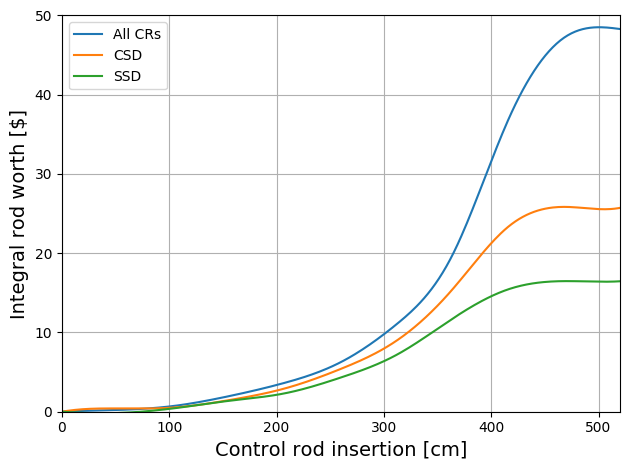
\includegraphics[width=\textwidth]{integ.png}
	\vspace{-0.5in}
	\caption{Integral CRW of all CRs, CSD, and SSD clusters (CRs made of B$_4$C-90).} 
	\label{fig:integ}
\end{figure}
\begin{figure}
	\centering
	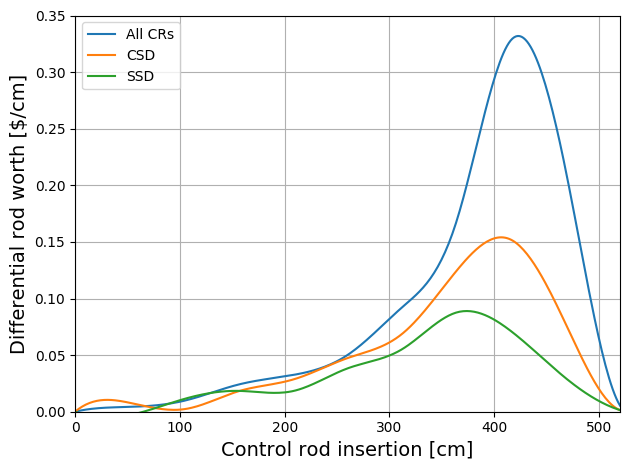
\includegraphics[width=\textwidth]{diff.png}
	\vspace{-0.5in}
	\caption{Differential CRW of all CRs, CSD, and SSD clusters (CRs made of B$_4$C-90).} 
	\label{fig:diff}
\end{figure}
\begin{figure}
	\centering
	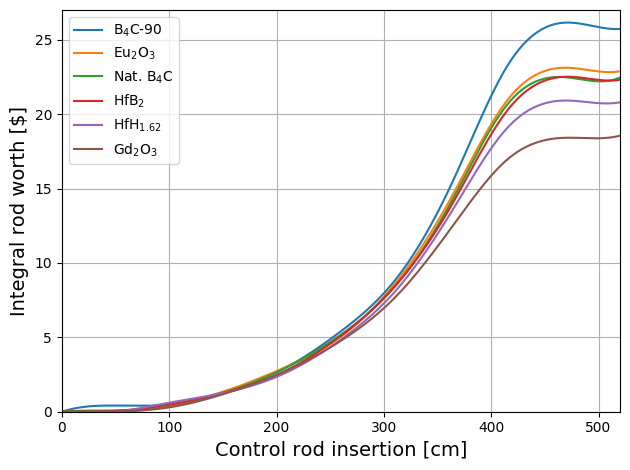
\includegraphics[width=\textwidth]{CSD.png}
	\vspace{-0.5in}
	\caption{Integral CRW of CSD clusters for various absorbing materials.} 
	\label{fig:CSD}
\end{figure}
\FloatBarrier
%\section{Discussion}
% This should explore the significance of the results of the work, not repeat
% them. A combined Results and Discussion section is often appropriate. Avoid
% extensive citations and discussion of published literature.
Short 2-3 paragraph discussion. This will emphasize:
\begin{itemize}
  \item Discuss reason of spectral shift (heavy \gls{FP} accumulation, Pu isotopes).
  \item Neutron spectral shift which causes safety parameters worsening.  
  \item Couple words about power profile.
\end{itemize}

%\FloatBarrier
\section{Conclusion} \label{Conclusion}
In the current work, we proposed a reactivity control system design for the 
Single-fluid Double-zone Thorium-based Molten Salt Reactor (SD-TMSR). The 
design has been evaluated at the startup for the full-core geometry using the
SERPENT-2 Monte-Carlo code. We considered three startup fuel salt compositions:
(1) $^{232}$Th as fertile and $^{233}$U as fissile material; 
(2) $^{232}$Th and Pu, extracted from \gls{LWR} \gls{SNF}; (3) 
$^{232}$Th and TRU, extracted from \gls{LWR} \gls{SNF}.

The excess reactivity $\rho_e$ is calculated at zero burnup when all CRs are 
fully withdrawn. The $\rho_e$ for $^{233}$U, reactor-grade Pu, and 
TRU are $1.65\pm0.04$ $\$$, $4.11\pm0.02$ $\$$, and $15.38\pm0.04$ $\$$, 
respectively.

Six different absorbing materials are considered in this work:
natural B$_4$C, B$_4$C-90 (boron is enriched to 90\% $^{10}$B), HfB$_2$, 
HfH$_{1.62}$, Eu$_2$O$_3$, and Gd$_2$O$_3$. Enriched B$_4$C-90 has the largest 
absorption ability, while Gd$_2$O$_3$ has the lowest absorption compared with 
the other absorbing materials in this study. Both Control Safety Devices (CSD)
and Shutdown Safety Devices (SSD) clusters are 
separately able to shut down the reactor initially loaded with $^{233}$U and 
reactor-grade Pu regardless of the absorbing material type. However, only SSD 
clusters made of B$_4$C-90 are able to shut down the SD-TMSR initially loaded 
with TRU from \gls{LWR}. The reason for this is the much larger 
absorption cross section of $^{10}$B in the relatively soft neutron energy 
spectrum of the SD-TMSR core started with TRU.

In case of malfunction of the other CR clusters (e.g., stuck in the upper 
position), the outer ring of the CSD failed to counteract the excess 
reactivity of the core initially loaded with reactor-grade Pu and TRU elements.
However, the worth of the outer ring of the CSD is sufficient 
to compensate the excess reactivity for the core refueled by $^{233}$U.

All absorbing materials provide an adequate shutdown margin for the SD-TMSR 
core that initially loaded with $^{233}$U and reactor-grade Pu. However, the 
shutdown margins for TRU case are negative or slightly positive (in B$_4$C-90 
case).

The amplification factor (A$_{CRi}$) results show that the CSD, SSD, CSD inner ring, and SSD1 are slightly amplified due to the anti-shadowing effects. The strongest anti-shadowing effect has observed in SSD4 and CSD9 clusters that are located at the boundary between the core zones with different moderator-to-fuel ratio.

The insertion of CRs deforms the radial flux shape in certain positions, i.e., around CRs. This shifts the neutron flux from the core center towards the periphery.

The integral and differential CR worth are calculated for three 
different systems: all CRs, CSD, and SSD systems. The results show 
that all absorbing materials have almost the same integral rod worth in the 
upper half of the core. Further insertion of the CRs shows the unique 
absorption characteristics of each material.

Finally, the proposed design of CRs successfully control the excess reactivity and enhance the safety aspects of the SD-TMSR.

\section{Future work}
In Part II of this research effort, we will evaluate the effect of fuel salt 
burnup on the CRW. The depleted fuel composition will be obtained using a
SERPENT-2 online reprocessing subroutine and 
batch-wise tool SaltProc \cite{rykhlevskii_milestone_2019}. Additionally, the authors intend to investigate 
kinetic parameters' (effective delayed neutron fraction $\beta_{eff}$ and 
effective delayed neutron precursor decay constant $\lambda_{eff}$) evolution 
during the SD-TMSR operation. These parameters are crucial for accident 
transient analysis, which will be performed using Moltres 
\cite{lindsay_introduction_2018}, a multi-physics application for liquid-fueled MSR 
simulation which takes into account the neutron precursors drift.

\section{Declaration of Competing Interest}

The authors declare that they have no known competing financial interests or personal relationships that could have appeared to influence the work reported in this paper.

\FloatBarrier
\section{Acknowledgments}

Osama Ashraf would like to thank the Egyptian Ministry of Higher Education (MoHE), as well as MEPhI's Competitiveness Program for providing financial support for this research. The facility and tools needed to conduct this work were supported by MEPhI.

The authors contributed to this work as described below.

Osama Ashraf conceived and designed the simulations, wrote the paper, prepared figures 
and/or tables, performed the computation work, and reviewed drafts of the paper.

Andrei Rykhlevskii conceived and designed the simulations, wrote the paper, prepared figures 
and/or tables, performed the computation work, and reviewed drafts of the paper. Andrei Rykhlevskii 
is supported by  DOE ARPA-E MEITNER program award DE-AR0000983. 

G. V. Tikhomirov directed and supervised the work, conceived and designed the simulations and reviewed drafts of the paper. Prof. Tikhomirov is supported by Rosatom, he is Deputy Director of the Institute of Nuclear Physics and Engineering MEPhI. Board member of Nuclear society of Russia.

Kathryn D. Huff supervised the work, conceived and contributed to conception of the simulations, and reviewed drafts of the paper.  Prof. Huff is supported by the Nuclear Regulatory Commission Faculty Development Program, the National Center for Supercomputing Applications, the International Institute for Carbon Neutral Energy Research (WPI-I2CNER), 
sponsored by the Japanese Ministry of Education, Culture, Sports, Science and Technology, and  DOE ARPA-E MEITNER program award DE-AR0000983.

This research is part of the Blue Waters sustained-petascale computing project, 
which is supported by the National Science Foundation (awards OCI-0725070 and 
ACI-1238993) and the state of Illinois. Blue Waters is a joint effort of the 
University of Illinois at Urbana-Champaign and its National Center for 
Supercomputing Applications 

\FloatBarrier
\bibliographystyle{elsarticle-num}
\bibliography{2019-CRs}
\newpage
%\appendix
%\section{Feed rates for all cases}
\setcounter{table}{0}  
\begin{table}[ht!]
	\centering
	\caption{The refueling table for Th/$^{233}$U case.} 
	\vspace{1ex}
	\begin{tabularx}{\textwidth}{|p{1.5cm}|b|p{2.9cm}|}
		\hline
		\textbf{Material} & \textbf{Feed rate} & \textbf{Feed 
			constant$^{\star}$} $\lambda_{e}$ $[s^{-1}]$ \\
		\hline
		$^{232}$Th        &  1.842 [kg/day], first 90 [d] & 1.500E-09 \\
		&  2.511 [kg/day], from 90 to 1550 [d] & 		2.045E-09 \\
		&  2.456 [kg/day], from 1550 to 3010 [d] & 		2.000E-09 \\
		&  2.321 [kg/day], from 3010 to 5930 [d]& 		1.890E-09	\\
		&  2.241 [kg/day], from 5930 to 7390 [d] &		1.825E-09	\\
		&  2.186 [kg/day], from 7390 to 12500 [d] &		1.780E-09	\\
		&  2.118 [kg/day], from 12500 to 15420 [d] &	1.725E-09	\\
		&  2.136 [kg/day], from 15420 to 18340 [d]&		1.740E-09		\\
		&  2.063 [kg/day], from 18340 to 21900 [d]&		1.680E-09	 \\ 
		\hline
		$^{233}$U & 2.619 [kg/day], first 90 [d]	&   6.400E-09  \\
		& 2.009 [kg/day],  form 90 to 1550 [d] &	4.910E-09 \\
		& 1.944 [kg/day], from 1550 to 3010 [d] &	4.750E-09 \\
		& 1.826 [kg/day],  from 3010 to 5930 [d] &	4.460E-09 \\
		& 1.811 [kg/day],  from 5930 to 7390[d] &	4.425E-09 \\
		& 1.744 [kg/day], from 7390 to 12500 [d] &	4.260E-09 \\
		& 1.699 [kg/day], from 12500 to 18340 [d]	& 4.150E-09 \\
		& 1.657 [kg/day], from 18340 to 21900 [d]	& 4.050E-09 \\
		\hline
	\end{tabularx}
	\begin{tablenotes}
		\small
		\item  $^{\star}$ Feed constant is the mass fraction of fertile or fissile nuclides ($^{232}$Th or $^{233}$U) transferred from the external storage to the core per second.
	\end{tablenotes}
	\label{tab:table8}
\end{table}	
\newpage
\begin{longtable}{|p{0.12\textwidth}|p{.53\textwidth}|p{.24\textwidth}|}
	%\begin{tabularx}{\textwidth}{|p{1.5cm}|b|p{2.9cm}|}
	\caption{The refueling table for reactor-grade Pu case.} 
	\vspace{-0.2in}
	\label{tab:table9}
	\endfirsthead
	\endhead
	\hline
	\textbf{Material} & \textbf{Feed rate} & \textbf{Feed 
		constant} $\lambda_{e}$ $[s^{-1}]$ \\
	\hline
	Pu        &  3.028 [kg/day], first 365 [d] & 1.71E-08 \\
	&  3.099 [kg/day], from 365 to 730 [d] & 		1.75E-08 \\
	&  3.276 [kg/day], from 730 to 1095 [d] & 		1.85E-08 \\
	&  3.188 [kg/day], from 1095 to 1460 [d]& 		1.80E-08	\\
	&  3.158 [kg/day], from 1460 to 1825 [d] &		1.78E-08	\\
	& 3.034 [kg/day], from 1825 to 2190 [d] &		1.71E-08	\\
	& 3.299   [kg/day], from 2190 to 2555 [d] &	1.86E-08	\\
	&  2.581  [kg/day], from 2555 to 2920 [d]&		1.46E-08		\\
	&  2.484  [kg/day], from 2920 to 3285 [d]&		1.40E-08	 \\ 
	&  2.444  [kg/day], from 3285 to 3650 [d]&		1.38E-08	 \\ 
	&   2 [kg/day], from 3650 to 4015 [d]&		1.13E-08	 \\ 
	&  2.532  [kg/day], from 4015 to 5110 [d]&		1.43E-08	 \\
	&  2.568  [kg/day], from 5110 to 6205 [d]&		1.45E-08	 \\
	&  2.515  [kg/day], from 6205 to 6935 [d]&		1.42E-08	 \\
	& 2.483 [kg/day], from 6935 to 7300 [d]&		1.40E-08	 \\
	&  2.417  [kg/day], from 7300 to 7665 [d]&		1.37E-08	 \\
	&  2.134  [kg/day], from 7665 to 8030 [d]&		1.21E-08	 \\
	&  2.786  [kg/day], from 8030 to 8395 [d]&		1.57E-08	 \\
	&   2.679 [kg/day], from 8395 to 8760 [d]&		1.51E-08	 \\
	&  2.355   [kg/day], from 8760 to 9490 [d]&		1.33E-08	 \\
	&  2.727  [kg/day], from 9490 to 9855 [d]&		1.54E-08	 \\
	&  2.484  [kg/day], from 9855 to 10220 [d]&		1.40E-08	 \\
	& 2.502  [kg/day], from 10220 to 10585 [d]&		1.41E-08	 \\
	& 2.520  [kg/day], from 10585 to 10950 [d]&		1.42E-08	 \\
	&  2.538  [kg/day], from 10950 to 11315 [d]&		1.43E-08	 \\
	&  2.555  [kg/day], from 11315 to 13140 [d]&		1.44E-08	 \\
	&  2.573  [kg/day], from 13140 to 14600 [d]&		1.45E-08	 \\
	&  2.520  [kg/day], from 14600 to 16425 [d]&		1.42E-08	 \\
	& 2.396  [kg/day], from 16425 to 17155 [d]&		1.35E-08	 \\
	&  2.414 [kg/day], from 17155 to 17885 [d]&		1.36E-08	 \\
	& 2.573 [kg/day], from 17885 to 19710 [d]&		1.45E-08	 \\
	&  2.697 [kg/day], from 19710 to 20075 [d]&		1.52E-08	 \\
	&  2.573 [kg/day], from 20075 to 21170 [d]&		1.45E-08	 \\
	&  2.39 [kg/day], from 21170 to 21900 [d]&		1.35E-08	 \\
	\hline
	$^{233}$U &  0.531 [kg/day], from 365 to 1095  [d]	&   3.00E-09  \\
	&  0.690 [kg/day],  form 1095 to 1460 [d] &	3.90E-09 \\
	& 0.673 [kg/day], from 1460 to 2190 [d] &	3.80E-09 \\
	& 0.708  [kg/day], from 2190 to 2555 [d] &	4.00E-09 \\
	& 0.921  [kg/day], from 2555 to 2920 [d] &	5.20E-09 \\
	&   1.053  [kg/day], from 2920 to 3650 [d] &	5.95E-09 \\
	&  1.027 [kg/day], from 3650 to 4015 [d] &	5.80E-09 \\
	&  1.080  [kg/day], from 4015 to 5110 [d] &	6.10E-09 \\
	&  1.043  [kg/day], from 5110 to 7665 [d] &	5.89E-09 \\
	&  0.867  [kg/day], from 7665 to 8760 [d] &	4.90E-09 \\
	&  0.885  [kg/day], from 8760 to 9125 [d] &	5.00E-09 \\
	&  0.867  [kg/day], from 9125 to 10220 [d] &	4.90E-09 \\
	&  0.850 [kg/day], from 10220 to 10585 [d] &	4.80E-09 \\
	& 0.832  [kg/day], from 10585 to 10950 [d] &	4.70E-09 \\
	& 0.779   [kg/day], from 10950 to 12410 [d] &	4.40E-09 \\
	& 0.708  [kg/day], from 12410 to 13870 [d] &	4.00E-09 \\
	&  0.637  [kg/day], from 13870 to 17885 [d] &	3.60E-09 \\
	&  0.549  [kg/day], from 17885 to 20440 [d] &	3.10E-09 \\
	& 0.531 [kg/day], from 20440 to 21900 [d] &	3.00E-09 \\
	\hline
	
\end{longtable}	
\newpage
\begin{longtable}{|p{0.12\textwidth}|p{.53\textwidth}|p{.24\textwidth}|}
	%\begin{tabularx}{\textwidth}{|p{1.5cm}|b|p{2.9cm}|}
	\caption{The refueling table for TRU case.} 
	\vspace{-0.2in}
	\label{tab:table10}
	\endfirsthead
	\endhead
	\hline
	\textbf{Material} & \textbf{Feed rate} & \textbf{Feed 
		constant} $\lambda_{e}$ $[s^{-1}]$ \\
	\hline
	TRU        &  2.125 [kg/day], first 365 to 1095  [d] & 1.20E-08 \\
	&  2.302  [kg/day], from 1095 to 1825 [d] & 		1.30E-08 \\
	&  2.125  [kg/day], from 1825 to 2920 [d] & 		1.20E-08 \\
	&  1.9488 [kg/day], from 2920 to 4015 [d]& 		1.10E-08	\\
	&  2.479 [kg/day], from 4015 to 4380 [d] &		1.40E-08	\\
	&  1.948 [kg/day], from 4380 to 4745 [d] &		1.10E-08	\\
	&  2.125   [kg/day], from 4745 to 5110 [d] &	1.20E-08	\\
	&  1.948   [kg/day], from 5110 to 6935 [d]&		1.10E-08		\\
	&  2.479  [kg/day], from 6935 to 7300 [d]&		1.40E-08	 \\ 
	&  1.771   [kg/day], from 7300 to 7665 [d]&		1.00E-08	 \\ 
	&  1.948   [kg/day], from 7665 to 8030 [d]&		1.10E-08	 \\ 
	&  1.594   [kg/day], from 8030 to 8395 [d]&		0.90E-08	 \\
	&  2.125   [kg/day], from 8395 to 8760 [d]&		1.20E-08	 \\
	&  1.771  [kg/day], from 8760 to 9125 [d]&		1.00E-08	 \\
	& 2.125  [kg/day], from 9125 to 9490 [d]&		1.20E-08	 \\
	&  2.479  [kg/day], from 9490 to 9855 [d]&		1.4E-08	 \\
	&   2.036 [kg/day], from 9855 to 10220 [d]&		1.15E-08	 \\
	&  1.594 [kg/day], from 10220 to 10585 [d]&		0.90E-08	 \\
	&   1.771  [kg/day], from 10585 to 11680 [d]&		1.00E-08	 \\
	&  1.859   [kg/day], from 11680 to 12045 [d]&		1.05E-08	 \\
	& 2.214    [kg/day], from 12045 to 12410 [d]&		1.25E-08	 \\
	&  1.771   [kg/day], from 12410 to 13140 [d]&		1.00E-08	 \\
	&  2.479  [kg/day], from 13140 to 13505 [d]&		1.40E-08	 \\
	&  1.771 [kg/day], from 13505 to 13870 [d]&		1.00E-08	 \\
	& 1.594   [kg/day], from 13870 to 14235 [d]&		0.90E-08	 \\
	&  1.771   [kg/day], from 14235 to 14600 [d]&		1.00E-08	 \\
	& 1.948  [kg/day], from 14600 to 14965 [d]&		1.10E-08	 \\
	&  1.771   [kg/day], from 14965 to 17155 [d]&		1.00E-08	 \\
	&  1.416  [kg/day], from 17155 to 17520 [d]&		0.80E-08	 \\
	&  2.302  [kg/day], from 17520 to 17885 [d]&		1.30E-08	 \\
	& 1.594  [kg/day], from 17885 to 18250 [d]&		0.90E-08	 \\
	&   1.771 [kg/day], from 18250 to 20440 [d]&		1.00E-08	 \\
	&  1.594  [kg/day], from 20440 to 21170 [d]&		0.90E-08	 \\
	&  1.771 [kg/day], from 21170 to 21900 [d]&		1.00E-08	 \\
	\hline
	$^{233}$U &  1.066 [kg/day], first 365  [d]	&   6.02E-09  \\
	& 1.177 [kg/day],  form 365 to 1095 [d] &	6.65E-09 \\
	&  1.160 [kg/day], from 1095 to 1460 [d] &	6.55E-09 \\
	& 1.142   [kg/day], from 1460 to 2190 [d] &	6.45E-09 \\
	& 1.124  [kg/day], from 2190 to 2920 [d] &	6.35E-09 \\
	& 1.107 [kg/day], from 2920 to 4015 [d] &	6.25E-09 \\
	&  1.089 [kg/day], from 4015 to 4745 [d] &	6.15E-09 \\
	&  1.071  [kg/day], from 4745 to 5475 [d] &	6.05E-09 \\
	& 1.053  [kg/day], from 5475 to 6570 [d] &	5.95E-09 \\
	&  1.036  [kg/day], from 6570 to 7300 [d] &	5.85E-09 \\
	&  1.018   [kg/day], from 7300 to 8030 [d] &	5.75E-09 \\
	&  1   [kg/day], from 8030 to 9125 [d] &	5.65E-09 \\
	&  0.983 [kg/day], from 9125 to 9855 [d] &	5.55E-09 \\
	&  0.965  [kg/day], from 9855 to 10950 [d] &	5.45E-09 \\
	&   0.947  [kg/day], from 10950 to 12045 [d] &	5.35E-09 \\
	& 0.929  [kg/day], from 12045 to 12775 [d] &	5.25E-09 \\
	&  0.912   [kg/day], from 12775 to 13505 [d] &	5.15E-09 \\
	&   0.894  [kg/day], from 13505 to 14600 [d] &	5.05E-09 \\
	&  0.876 [kg/day], from 14600 to 15330 [d] &	4.95E-09 \\
	& 0.859   [kg/day], from 15330 to 16425 [d] &	4.85E-09 \\
	&  0.841 [kg/day], from 16425 to 17155 [d] &	4.75E-09 \\
	&  0.823 [kg/day], from 17155 to 18250 [d] &	4.65E-09 \\
	&  0.805 [kg/day], from 18250 to 19345 [d] &	4.65E-09 \\
	& 0.788  [kg/day], from 19345 to 20440 [d] &	4.45E-09 \\
	&  0.770 [kg/day], from 20440 to 21535 [d] &	4.35E-09 \\
	& 0.752 [kg/day], from 20440 to 21900 [d] &	4.25E-09 \\
	\hline
\end{longtable}
\end{document}
